% Revamped version for Demography focusing on method

\documentclass[12pt,letterpaper]{article}

\usepackage{amsmath}
\usepackage{fontspec}
\setromanfont[Ligatures=TeX]{TeX Gyre Pagella}
\usepackage{unicode-math}
\setmathfont{TeX Gyre Pagella Math}
\usepackage[title]{appendix}
\usepackage[margin=1.0in]{geometry}
\usepackage[figuresleft]{rotating}
\usepackage[longnamesfirst]{natbib}
\usepackage{dcolumn}
\usepackage{booktabs}
\usepackage{multirow}
\usepackage[flushleft]{threeparttable}
\usepackage{setspace}
\usepackage[justification=centering]{caption}
\usepackage[font=scriptsize]{subfig}
\usepackage[xetex,colorlinks=true,linkcolor=black,citecolor=black,urlcolor=black]{hyperref}
\usepackage{adjustbox}
\usepackage{xfrac}
\usepackage{placeins}


% \bibpunct{(}{)}{;}{a}{}{,}
\newcommand{\mco}[1]{\multicolumn{1}{c}{#1}}
\newcommand{\mct}[1]{\multicolumn{2}{c}{#1}}
\newcommand{\mcth}[1]{\multicolumn{3}{c}{#1}}
\newcommand{\X}{$\times$ }
\newcommand{\hs}{\hspace{15pt}}

% Attempt to squeeze more floats in
\renewcommand\floatpagefraction{.9}
\renewcommand\topfraction{.9}
\renewcommand\bottomfraction{.9}
\renewcommand\textfraction{.1}
\setcounter{totalnumber}{50}
\setcounter{topnumber}{50}
\setcounter{bottomnumber}{50}


%------------------------------------------------------------------------


\title{Birth Spacing in the Presence of Son Preference and Sex-Selective Abortions:
India's Experience over Four Decades%
\protect\thanks{%
I am grateful to Andrew Foster and Darryl Holman for discussions about the method.
I owe thanks to Shelly Lundberg, Daniel Rees, David Ribar, 
Hendrik Wolff, seminar participants at University of Copenhagen, University of Michigan, 
University of Washington, University of Aarhus, the Fourth 
Annual Conference on Population, Reproductive Health, 
and Economic Development, and the Economic Demography Workshop for helpful 
suggestions and comments.
I would also like to thank Nalina Varanasi for research assistance.
Support for development of the method from the University of Washington Royalty 
Research Fund and the Development Research Group of the World Bank is gratefully 
acknowledged.
The views and findings expressed here are those of the author and
should not be attributed to the World Bank or any of its member countries.
Partial support for this research came from a Eunice Kennedy Shriver National
Institute of Child Health and Human Development research infrastructure grant,
5R24HD042828, to the Center for Studies in Demography and Ecology at the
University of Washington.
}
}

\author{Claus C P\"ortner\\
    Department of Economics\\
    Albers School of Business and Economics\\
    Seattle University, P.O. Box 222000\\
    Seattle, WA 98122\\
    \href{mailto:claus@clausportner.com}{\texttt{claus@clausportner.com}}\\
    \href{http://www.clausportner.com}{\texttt{www.clausportner.com}}\\
    \& \\
    Center for Studies in Demography and Ecology \\
    University of Washington\\ \vspace{2cm}
    }

\date{December 2018}


%------------------------------------------------------------------------


\begin{document}
\graphicspath{{../figures/}}
\DeclareGraphicsExtensions{.eps,.jpg,.pdf,.mps,.png}

\setcounter{page}{-1}
\maketitle
\thispagestyle{empty}

% \setcounter{page}{0}


\newpage
\thispagestyle{empty}
\doublespacing

\begin{abstract}

% Demography abstract
\noindent 
Strong son preference is typically associated with shorter birth spacing in the absence of 
sons, but access to sex selection has the potential to reverse this pattern because each 
abortion extends spacing by six to twelve months. 
I introduce an empirical method that simultaneously accounts for how sex selection 
increases both birth spacing and the likelihood of a son. 
Using the four rounds of India's National Family and Health Surveys, I show that birth 
intervals increased substantially over the last four decades, with the most significant
increases among women most likely to use sex selection.
Specifically, well-educated women with no boys now have significantly longer birth
intervals, and more male-biased sex ratios, than similar women with boys. 
Women with no education still follow the standard pattern of short average spacing when 
they have girls and little evidence of sex selection, with medium-educated women showing 
mixed results.
Furthermore, the traditional pattern of longer average spacing with sons appears to arise 
not from fewer very short birth intervals, but rather from the upper end of the distribution.


\noindent JEL: J1, O12, I1
\noindent Keywords: India, prenatal sex determination, censoring, competing risk, non-proportional hazard
\end{abstract}

\newpage


%------------------------------------------------------------------------

\section{Introduction\label{sec:intro}}

Birth spacing has long served as a measure of son preference, with strong
son preference associated with shorter birth intervals the
fewer sons a family has \citep{ben-porath76b,Leung1988}.
However, the introduction of prenatal sex determination potentially 
changed the relationship between son preference and birth spacing.
The stronger the son preference, the more likely couples are to resort to sex-selective 
abortions, and each abortion increases the interval between births by six to twelve 
months.%
\footnote{
The increase consists of three parts.
First, starting from the abortion, the uterus needs at 
least two menstrual cycles to recover;  otherwise, the likelihood 
of spontaneous abortion increases substantially \citep{zhou00b}.
The second part is the waiting time to conception, which is between 
one and six months \citep{Wang2003}.
Finally, sex determination tests are reliable only from three months 
of gestation onwards.
}
Hence, longer birth intervals in the absence of sons, which previously would be taken as 
an indicator of lower son preference, may now instead arise because couples with a strong 
son preference use sex selection.

Here, I examine how birth spacing in India has changed over time and across 
groups with the introduction of sex selection.
I introduce an empirical method that directly incorporates the effects of 
sex-selective abortions on birth intervals
\emph{and} 
the likelihood of a son. 
The method can be used to analyze both situations with and without prenatal
sex selection.
I apply the method to birth histories of Hindu women, using data from the four
India's National Family and Health Surveys (NFHS), covering the period 
1972 to 2016. 


% [Why India?]
India is a particularly compelling case with its long history of male preference, 
especially in the northern states \citep{Kishor1993,murthi95,arnold98}.
Mortality risk is higher for females than males for most ages groups, resulting in
an almost continuous increase in India's overall ratio of males to females 
over the last century \citep{dyson01,Navaneetham2011,Bongaarts2015}.
Differential stopping behavior is widespread, with an additional child more likely the
fewer sons a family has 
\citep{repetto72,Das1987,Arnold1997,arnold98,clark00,Basu2010,Barcellos2014}.%
\footnote{
Other countries show a similar pattern
\citep[see, for example,][]{larsen98,filmer09,Altindag2016}.
}
Furthermore, fertility has declined substantially, to the point where it is now at, or even 
below, replacement in some areas 
\citep{Guilmoto2013,Dharmalingam2014,International-Institute-for-Population-Sciences-IIPS2017}.
The combination of falling fertility, strong son preference, and expanding access to 
prenatal sex determination has lead to dramatic increases in the males-to-females ratio at 
birth over the last three decades
\citep{das_gupta97,Sudha1999,Arnold2002,retherford03b,jha06,Guilmoto2009a,Guilmoto2012,Bongaarts2013,Portner2015b,Jayachandran2017}.


% [Why spacing?] 
There are four main reasons for examining birth spacing and how it changes with 
access to sex selection.
First, researchers have made extensive use of birth spacing as a measure of son preference, 
and it is critical to understand to what extent spacing is still a useful measure of son 
preference.
For example, in Bangladesh, India, and Vietnam, having more boys, and particularly having 
a boy as the last-born child, significantly increase the duration to next birth,
\citep{Haughton1995,Haughton1996,Rahman1993,Bhalotra2008,Kumar2016,Soest2018}.%
\footnote{
Ethnic Indians in South Africa also show a longer duration after the birth of a 
son than after a daughter \citep{Gangadharan2003}.
}
Outside Asia, the evidence is more mixed, with North Africa showing shorter spacing in the 
absence of sons, while a similar pattern does not exist in Sub-Saharan Africa 
\citep{Rossi2015}.

Second, birth spacing can affect children's short and long-term outcomes.
Most of the research finds a negative impact of short spacing on child health, especially 
for very short intervals of 18 months or less \citep{Conde-Agudelo2006,Conde-Agudelo2012}.
There is evidence in countries as diverse as Bangladesh, Brazil, El Salvadore, India,
and Pakistan of worse health outcomes and a higher mortality risk the shorter the birth
interval
\citep{Cleland1984,Curtis1993,Whitworth2002,Bhargava2003,Rutstein2005,Bhalotra2008,Davanzo2008,Maitra2008,Makepeace2008,Gribble2009,Jayachandran2011,Saha2013,Jayachandran2017a,Ghosh2018}.
Most of the evidence on longer-term outcomes come from Western countries.
In the US, for example, a longer interval between births increases the older, but not the
younger, sibling's test scores \citep{Buckles2012}.
Furthermore, close spacing appears to increase the risk of dropping out of
high school and lower the probability of attending a post-secondary school in both the
US and Sweden \citep{Powell1993,Pettersson-Lidbom2009}.%
\footnote{
However, recent results from Sweden show no relationship between birth spacing, even if 
very short, and outcomes such as years of education completed, earnings, and unemployment 
\citep{Barclay2017}.
}

Third, the mother may also be affected by the length of the birth intervals, although 
reviews of the literature show mixed results on mother's anthropometric status 
\citep{Dewey2007,Conde-Agudelo2012}.
For India, there is, however, evidence that women with first-born girls are more likely to 
have anemia, possibly because short birth spacing can resulting in maternal depletion 
\citep{Milazzo2018}.
In Western countries, a longer interval between births has positive effects on long-term 
labor market outcomes, such as participation and income \citep{Gough2017,Karimi2014}.

Finally, we know less about what determines spacing behavior in developing countries than 
in developed countries, and with declining fertility and increasing numbers of women 
entering the labor force, understanding how couples make timing decisions is necessary 
for the design of suitable policies \citep{Portner2018}.%
\footnote{
It is clear that birth spacing does respond to policies in both developed and 
developing countries \citep{Pettersson-Lidbom2009,Todd2012,Meckel2015,Ghosh2018}.
}
Even the effects of access to contraceptive and declining fertility on spacing are unclear.
On the one hand, access to contraceptives allows women to avoid too short spacing between 
birth.
On the other hand, increased reliability of access and effectiveness of contraceptives can 
lead to shorter intervals between births if women used to have longer spacing to avoid
having too many children by accident \citep{Keyfitz1971,Heckman1976}.
These two counteracting effects may explain why better-educated women have shorter spacing 
than less educated women in some instances but not in others and why finding statistically 
significant effects of contraception use on birth spacing is difficult 
\citep{Tulasidhar1993,Whitworth2002,Bhalotra2008,Yeakey2009,Kim2010,Soest2018}.%
\footnote{
In Matlab, the effect of son preference on birth spacing is stronger in areas with better 
access to family planning \citep{Rahman1993}.
Other evidence, however, points to families ability to time births, even in the absence
of modern contraceptives \citep{Jayachandran2011,Alam2018}.
}

% [Hypotheses / questions]
Despite the increasing use of sex selection, the critical impacts of spacing on outcomes 
for both mother and children, and the extensive use of spacing to measure son preference, 
there has so far been no systematic examination of what effect access to sex selection 
have on spacing.
I address three questions to remedy this shortcoming in the literature.

First, how did average birth intervals change over time for different groups and how do 
these changes relate to the use of sex selection?
The hypothesis is that in the absence of sex selection son preference leads to shorter 
spacing the fewer boys a family has, whereas son preference increases spacing the fewer 
boys a family has when prenatal sex selection is available, possibly to the point where
we observe a reversal of the standard spacing pattern.
Families with son preference who---for one reason or another---do not use prenatal sex 
selection likely continue to have shorter birth spacing.
Based on the prior literature on sex selection, I focus on how birth intervals have
changed for different education levels, urban or rural, and the sex composition of 
prior children.

Second, have the shapes of the survival curves changed?
Although examining average birth intervals helps us understand the overall changes in 
spacing behavior, it tells us little about how these changes came about.
For example, the motivations that lead to an increase in average spacing are different if 
the increase comes mainly from parents trying to avoid very short birth intervals or from 
continued use of sex selection to ensure a son.


There are four main results.
First, the intervals between births have increased for all education groups over the four 
decades.
These increases are larger the higher the parity and the higher the education 
level.
Second, those women who are most likely to use sex selection---well-educated women with no
sons---have seen the largest increases in birth intervals.
As a result, well-educated women now show a reversal of the traditional spacing 
pattern, with the longest birth intervals for women with no sons.
Third, women who are least likely to use sex selection, those with no education in
rural areas, still follow the standard pattern of short spacing when they have girls and 
little evidence of the use of sex selection.
Finally, the traditional pattern of longer average spacing with sons appear to arise from 
more very long intervals, rather than from fewer very short birth intervals; across 
education groups, there appears to be little difference in the likelihood of having a very 
short birth interval across sex compositions, especially for lower parities.


%------------------------------------------------------------------------------------

\section{Birth Spacing: Mechanisms and Findings}

This section provides a conceptual framework for understanding what determines  
birth spacing.
I first discuss the main determinants of spacing examined in the prior research, and 
then how son preference and sex selection fits into the spacing decisions.
Since sex selection and education are closely linked, I pay special attention to how 
education affects spacing.

In the simplest possible dynamic model of fertility, the spacing decision is trivial.
Assume that parents derive benefits from the presence of children, not their births, 
that spacing of children does impact parents' utility, 
and that the parents fully control when to have children. 
The optimal decision then is to have the children as early as possible 
\citep{Newman1988}.
The simplest model does not fit the observed spacing patterns, which suggests 
that one or more of the assumptions are wrong.

First, parents do not entirely control the timing of births, but rather decide on 
the levels of sexual activity and contraceptive effort, which, in turn, affect the 
likelihood of conceiving, while taking into account fecundity and their knowledge 
of and access to contraceptive technology.

Fecundity determinants, such as age and health of the mother, are, however, unlikely 
to be significant factors in how spacing changed over time or across education levels 
in India for the period covered.
Outside of direct famine conditions, women's health and nutritional status do not 
appear to affect spacing substantially \citep{Huffman1987,John1987,lindstrom99}.
The Maharashtra drought occurred in 1970--1973 and would, therefore, only impact the first
year or two of the data.
Furthermore, I only examine spacing up to parity fourth, and the age of the mother is,
therefore, unlikely to be a concern when it comes to fecundity, even though 
better-educated women are, on average, older when they marry. 

Despite a general belief that better access to and knowledge of contraception 
should lengthen average spacing, the empirical relationship between contraception 
use and birth spacing is ambiguous 
\citep{Tulasidhar1993,Whitworth2002,Bhalotra2008,Yeakey2009,Kim2010,Soest2018}.
This lack of evidence is consistent with the ambiguous theoretical effect of introducing 
modern contraceptives on birth spacing.
On the one hand, in the absence of high-efficacy contraceptive technologies, parents may 
try to avoid overshooting their desired number of children by spacing their children 
further apart than they would otherwise do.
Increased reliability of the access to and effectiveness of contraceptives then lead to 
shorter birth intervals because parents are more confident they can effectively
stop childbearing when they want \citep{Keyfitz1971,Heckman1976}.
On the other hand, through simple random variation, when contraceptives are ineffective, 
some birth intervals will be shorter than ideal, in the way discussed below.
With increased reliability of contraceptive efforts, parents can better avoid too short 
birth spacing, and average spacing should go up.

To further complicate the relationship between contraception and spacing, the ability 
to successfully use ``low efficacy'' contraceptive methods, such as the rhythm method, 
is increasing in education, while there is no difference across education levels 
when it comes to modern contraceptives such as pills or injectables \citep{Rosenzweig1989}.
Additionally, even in the absence of modern contraceptives, families appear able to 
time or at least postpone births when they have substantial enough incentive 
\citep{Jayachandran2011,Alam2018}.


Second, parents may care about the spacing between birth because of the 
potential effects of spacing on the children.%
\footnote{
In principle, the mother could also be affected, but the estimated impact on 
mothers' anthropometric status is mixed, and there appears to be no 
effect on mortality 
\citep{Ronsmans1998,Menken2003,Dewey2007,Conde-Agudelo2012}.
}
One theory is that child ``quality'' increases with spacing 
since parental attention per child increases
\citep{Zajonc1975,Zajonc1976,Razin1980}.
In this case, birth spacing should increase in family income, while the 
effect of maternal education is ambiguous since higher education, on the 
one hand, makes the mother's time spent out of the labor market more 
costly and on the other hand increases how productive the mother is 
in childrearing.
The evidence on spacing's effect on child quality measures such as IQ 
and education is, however, mixed for developed countries and non-existing 
for developing countries
\citep{Powell1993,Pettersson-Lidbom2009,Buckles2012,Barclay2017}.

For one crucial aspect of child quality---health and mortality---shorter spacing 
does lead to worse outcomes, especially for very short intervals of 24 months 
or less, although this effect decreases with maternal education
\citep{Whitworth2002,Conde-Agudelo2006,Conde-Agudelo2012,Molitoris2019}.%
\footnote{
The underlying mortality risk could also affect birth spacing, but
there is little empirical evidence for this 
\citep{Newman1983,Newman1988,Bhalotra2008}.
}
If parents realize short birth spacing increases their children's mortality risk, 
they likely prefer to space births further apart.
However, this effect should diminish with education level since women with 
secondary or tertiary education experience relatively low mortality risk for 
their children, even with very short spacing is associated.


Third, parents incur both direct and time costs when they have children, 
and economic considerations can, therefore, affect birth spacing 
\citep{Hotz1997,schultz97}.
I divide the economic factors into the effects of economies of scale and
the expected income trajectory of the husband and wife.

The expected effect of economies of scale in childrearing, which, for example, 
can arise because taking care of two young children does not take twice as much 
time as taking care of one child, is to shorten intervals between births
\citep{Vijverberg1982}.
To the extent that children require the mother to do less market work, parents 
can lower the cost of children by reducing birth spacing.
In this case, better-educated women will both have lower fertility and shorter
spacing than less-educated women because of their higher opportunity cost of time 
\citep{Ross1974,Newman1984}.
However, if the mother mainly works at home or as household income increases, there 
is less incentive to space children for this reason.

In the absence of perfect capital markets, theory predicts that the steeper 
the parents' lifetime income profile, the longer the spacing between births, 
which suggests that with economic development we should see a general increase 
in spacing across education groups and that this increase in spacing should be 
stronger with increasing education levels
\citep{Heckman1976,wolpin84,Newman1988}.
The idea is that although parents would prefer to have their children as early 
as possible to enjoy them for longer, there is also a direct cost to children.
Income is low early on, which means that the marginal utility of consumption is 
higher, making parents less willing to give up consumption to have a child, 
compare to later when they know that their income will be higher 
\citep{Newman1984,Happel1984}.

Finally, the discussion has so far assumed that children are identical---except 
for any differences that arise from spacing---but there is substantial evidence 
that the sex composition of previous children affects birth spacing, with the
absence of boys significantly decreasing the duration to next birth
\citep{Haughton1995,Haughton1996,Rahman1993,Bhalotra2008,Kumar2016,Soest2018}.
There is also evidence of differential stopping behavior, with an additional child 
more likely the fewer sons a family has 
\citep{repetto72,Das1987,Arnold1997,arnold98,clark00,Basu2010,Barcellos2014}.

If short spacing lowers the survival probability of the next child, as discussed above,
it is not, however, apparent that we should expect shorter spacing in the absence of boys.
There are two potential reasons why parents might still try to conceive sooner 
in the absence of boys.%
\footnote{
The significant differences in spacing by sex composition indicate that
parents control the timing of birth, at least to some extent.
In Matlab, the effect of son preference on birth spacing is stronger in 
areas with better access to family planning \citep{Rahman1993}.
}
One possibility is that parents do not realize that short spacing is potentially
detrimental to the next child's health, resulting in high mortality for both boys 
and girls born after short spacing across all households.

The other possibility is that parents realize that short spacing has adverse 
health effects, but their preference for sons is so strong that they are willing to 
divert substantial resources to the next child if it is a boy.
Assuming that these investments can compensate for the adverse effects,
we should see significant differences in mortality across sex for short-spacing 
children in the absence of boys.
If a son is born, his mortality risk should be substantially lower than expected 
for the spacing duration, and we should expect worse outcomes for the other 
children (all girls).
If a girl is born, there are two possible outcomes.
If parents treat all children/girls the same, we should see a slight worsening in 
health outcomes because fewer resources are available per child; 
if they do not, the last girl will have a much lower likelihood of surviving 
because the parents' incentive is to invest in their prior children rather than 
the new child.

With the adverse effects of shorter spacing strongly mitigated by higher education,
better-educated women can, in theory, have shorter spacing in the absence of a boy 
without substantial increasing mortality risk.
Differences in mortality outcomes across boys and girls are still possible,
but should not be as large as for less-educated women.

With the introduction of sex selection, parents can avoid the birth of girls, 
although at the cost of the procedure and having to wait longer until 
the next child if they abort the fetus.

Theory suggests that sex selection increases with lower desired fertility, and, for a 
given desired number of children, the higher the parity \citep{Portner2015b}.
The increased use of sex selection in India with education and in urban
areas is consistent with a lower desired fertility for both groups,
either because of the higher cost of children or because of other
changes in the preferred number of children
\citep{das_gupta97,retherford03b,jha06,Guilmoto2009a,Bongaarts2013,Portner2015b,
Jayachandran2017}.%
\footnote{
Stronger son preference could also contribute, but better-educated women 
have declining stated son preference over time \citep{bhat03,pande07}.
}

The higher the cost of prenatal sex determination and abortion, the less use we should 
see.
Similarly, any potential adverse effects on the mother and offspring 
from repeated abortions should also reduce the use of sex selection---provided that 
parents are aware of these costs.
Furthermore, the more abortions between births, the less the parents can take advantage 
of economies of scale.
Better-educated women tend to live in households with higher income, which better enables 
them to access prenatal sex determination and lowers the relative costs of using sex 
selection.

Given the increase in birth spacing with each abortion, parents may try to 
conceive even sooner to compensate for the potentially longer spacing and, 
thereby, still take advantage of economies of scale in childrearing.
Furthermore, if health outcomes for short spacing births have improved over 
time---as is likely---we should see an even stronger push toward shorter 
spacing for women using sex selection.

In summary, birth spacing is affected by female education through 
multiple pathways, with the main one of interest here the use of 
sex selection. 
But, to fully understand how sex selection affects spacing, we also 
need to understand the other changes that affect birth spacing over time.
The most likely factors are the changes in household income and 
wealth and the improvements in health as India has developed.
I, therefore, examine how female education and labor force 
participation has changed over time in India.

%------------------------------------------------------------------------------------

\section{Female Education and Labor Force Participation in India}

Female educational attainment has increased substantially over time.
Figure \ref{fig:education_over_time} shows the distribution of schooling by birth 
cohort for urban and rural women, 
twenty years or older, whether married or not, based on the four rounds of the NFHS.
The education groups are no education, one to seven years, and eight to eleven years,
and twelve years and above.

\begin{figure}[htpb]
\centering
\subfloat[Rural]{
    \begin{minipage}{0.49\textwidth}
        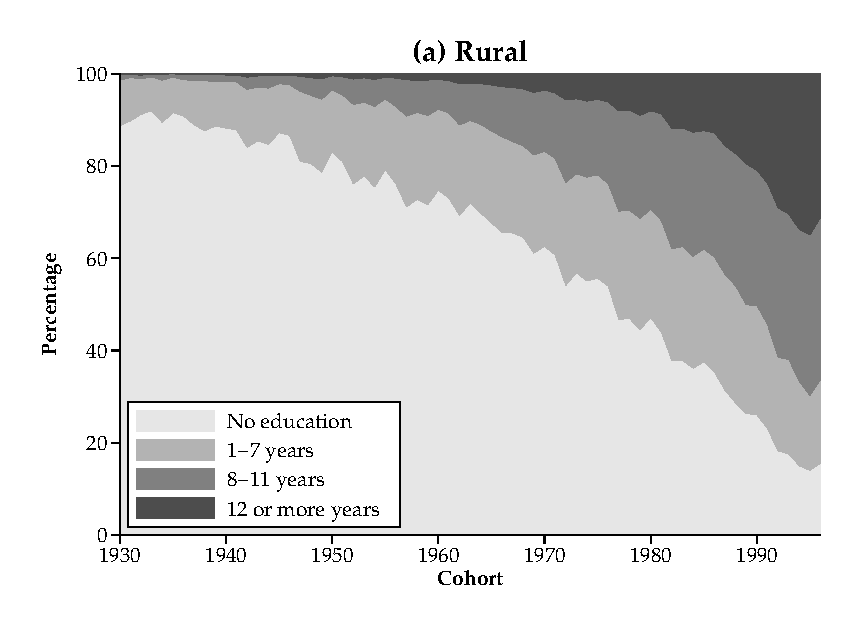
\includegraphics[width=\textwidth]{educ_over_time_rural}
    \end{minipage}
} 
\subfloat[Urban]{
    \begin{minipage}{0.49\textwidth}
        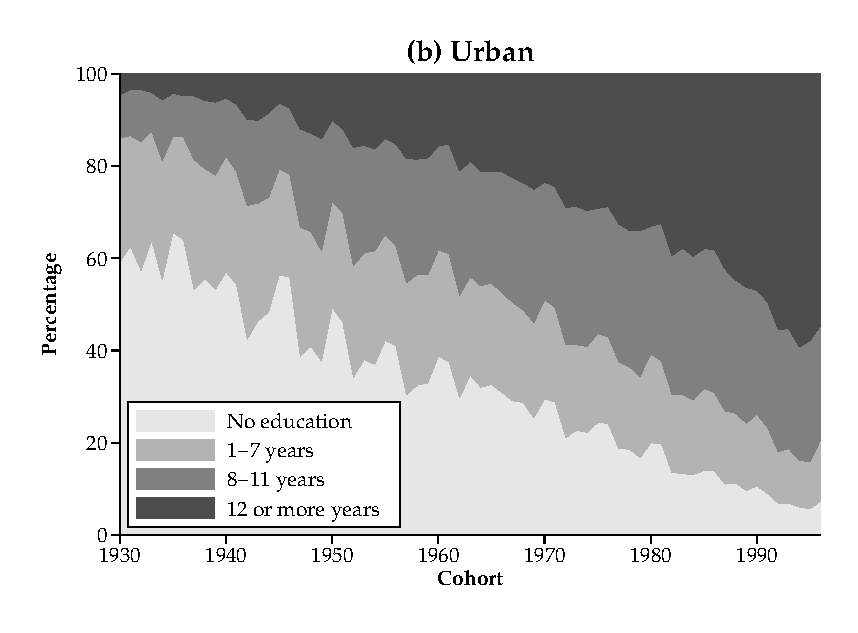
\includegraphics[width=\textwidth]{educ_over_time_urban} 
    \end{minipage}
}
\caption{Distribution of education by cohort for women twenty years or older at survey}
\label{fig:education_over_time}
\end{figure}


For rural areas, the percentage of women with no education has gone from around 90 percent
for the 1930s cohorts to less than 20 percent for the 1990s cohorts. 
The proportion of women with one to seven years of education has remained remarkably
constant at around ten percent.
The difference is made up by the women with eight or more years of education, who have
gone from almost zero for the 1930 cohort to more than sixty percent for the 1990s cohorts,
with about half in the eight to eleven years group and 
the other half in the twelve years or more group.

Female education is higher in urban areas than in rural areas.
Around sixty percent of urban women born in the 1930s had no education, 25 percent had
between one and seven years, about 10 had eight or more years of education, and only
five percent has twelve years or more.
The proportions with no education and one to seven years have both declined to just below 
ten percent for the latest cohort.
Although the proportion of women with eight to eleven years of education has increased
to about twenty, most of the increase in urban female education has come from the 
twelve plus group, which now account for more than half of all urban women.

Even as the level of female education has increased, the female labor force participation 
in both urban and rural areas has stagnated or decreased
\citep{Klasen2015,Afridi2018,Bhargava2018,Chatterjee2018, Bhargava2019}.
A decline in female labor force participation at the beginning of development is
consistent with the hypothesis of a U-shaped labor force participation as a country
develops \citep{Goldin1994}.
India's female labor force participation is, however, lower than most other
countries and more in line with countries in the Middle East and North Africa, and
does not yet show any signs of increasing
\citep{Klasen2015,Chatterjee2018}.

Theory predicts that increasing women's wages leads to higher labor force participation, 
while both a higher male income and stronger social restrictions on working, possibly in 
specific industries or jobs, reduce female labor supply \citep{Goldin1994}.
India's economy has grown substantially since the mid-seventies, with
an average annual growth rate of about 5.5 percent from 1978 to 2004 \citet{Bosworth2008}.
As a result, real wages for both men and women have almost doubled between 1987 and 2011 
\citep{Klasen2015}.
Despite the increases in wages and the higher female education, the mean male wage is
still close to 70 percent higher than the mean female wage \citep{Bhargava2018}.
Furthermore, the development in women's wages is not uniform across education 
levels \citep{Klasen2015,Bhargava2018}.
The real wages for women with middle school education or below have converged. 
For women with secondary education, the change over time depends on the sample used,
with some showing a substantial decline and others a modest increase.
Women with more than secondary education experienced an increased in their real 
wages, especially in cities.

After controlling for household characteristics and husband income, there is
still a U-shaped relationship between female education and labor supply with the
lowest labor force participation for women with secondary education \citep{Chatterjee2018}.
There are two possible explanations for this effect, both directly related to the strong
pro-male bias in India.
First, it becomes less socially acceptable for women to work in manual labor as their
education increases, and women are still mostly excluded from white-collar
employment despite robust economic growth \citep{Klasen2015,Chatterjee2018}.
Second, with increasing education, women's productivity at home also increases, especially
in the production of offspring human capital.
With relatively more boys born because of increased access to sex-selective 
abortions and an increasing male income, demand for better-educated women can 
increase, even if they do not participate in the labor market \citep{Behrman1999}.

Figure \ref{fig:work_by_survey} shows the percent of married women who are 
currently working at the time of the survey by age group and education level.
No other labor force participation question is consistently available across all 
four surveys. 
Because the question refers to currently working, the percentages will be lower 
than what other studies have found. 
Furthermore, since the question is asked only of married women, the overall female labor 
force participation might have developed differently, especially since many young, 
unmarried women have begun working in, for example, the business process 
outsourcing industry, which, in turn, has increased girls' schooling investments
\citep{Jensen2012}.

\begin{figure}[!htpb]
\centering
\rotatebox[origin=c]{90}{\small{40 Years or Older}}
\subfloat[Rural]{
    \begin{minipage}{0.45\textwidth}
        \includegraphics[width=\textwidth]{currently_working_rural_40}
    \end{minipage}
} 
\subfloat[Urban]{
    \begin{minipage}{0.45\textwidth}
        \includegraphics[width=\textwidth]{currently_working_urban_40} 
    \end{minipage}
}
\\
\rotatebox[origin=c]{90}{\small{30 to 39 Years Old}}
\subfloat[Rural]{
    \begin{minipage}{0.45\textwidth}
        \includegraphics[width=\textwidth]{currently_working_rural_30}
    \end{minipage}
} 
\subfloat[Urban]{
    \begin{minipage}{0.45\textwidth}
        \includegraphics[width=\textwidth]{currently_working_urban_30} 
    \end{minipage}
}
\\
\rotatebox[origin=c]{90}{\small{20 to 29 Years Old}}
\subfloat[Rural]{
    \begin{minipage}{0.45\textwidth}
        \includegraphics[width=\textwidth]{currently_working_rural_20}
    \end{minipage}
} 
\subfloat[Urban]{
    \begin{minipage}{0.45\textwidth}
        \includegraphics[width=\textwidth]{currently_working_urban_20} 
    \end{minipage}
}
\caption{Percentage of married women who were working at the time of the 
survey by age group and area of residence}
\label{fig:work_by_survey}
\end{figure}


The U-shaped relationship between education and working holds in most cases with 
the highest percent working for women with either no education or with twelve or 
more years and the lowest for women with eight to eleven years of education.
Women are more likely to report working if they live in rural than urban areas 
and the older they are.
Comparing 1992 and 2015, the percent of women who currently work has either 
remained roughly the same or decreased.
The cases were the numbers were higher in 1999 and 2006 than in 1992 or 2015 
are mostly based on small samples, such as rural women with twelve or more 
years of education in rural areas.

Almost all of the urban women who work receive either cash or a combination of 
cash and in-kind for their work (see Appendix Figure \ref{fig:work_cash_by_survey}). 
Rural women have become more likely to receive cash for their labor over time, 
and the better educated, the more likely they are to receive cash.

Despite this, women across all groups have become substantially more likely to 
work for a family member rather than for themselves or somebody else
(see Appendix Figure \ref{fig:work_family_by_survey}).
Hence, the lower likelihood of working stems mostly from women retracting from 
the general labor market and self-employment.

The increases in female educational attainment imply that access to education 
has expanded beyond the higher castes. 
However, ``Sanskritization'' implies that as lower castes females gain access to 
education and their husbands' income increases, the women adopt higher caste 
norms such as stronger son preference and a retraction from the formal labor 
market \citep{Srinivas1956,Chen1995,Abraham2013,Chatterjee2018}. 
``Sanskritization'' may also lead to an increased aversion to daughters, rather 
than just an increased preference for sons, which, in turn, lowers desired 
fertility \citep{Borooah2004}.

Hence, with substantial increases in husband income and a declining female labor force 
participation, I expect a push toward longer birth spacing over time, independent
of education levels, based on the income effects and the effects of spacing
on child outcomes in the theories above.
The declining percentage of women working suggests that the opportunity cost
effects with increasing education will not be strong enough to shorten the
birth spacing.

As desired fertility decreases with increasing education, I, furthermore, expect 
birth spacing to increase the most among the best-educated because of their 
use of sex selection and because of "Sanskritization" the changing composition 
of women in the better-educated group does not substantially change this 
group's use of sex selection.
Working in the opposite direction is that women with more education can space
their children closer together without substantially increasing child mortality risk.



\section{Estimation Strategy\label{sec:strategy}}

% Requirements for method and the intuition behind each:  
%  - Account for censoring (hazard model)
%  - Work both with and without sex selection (competing risk part)
%  - Allow for changes in use of sex selection within spell (flexible specification of baseline hazard ?)
%  - Capture that the shape of the hazard function differ across groups
%    (non-proportionality); needs a better description, maybe using example
%    of shorter spacing and/or use of sex selection. Differences in parity
%    progression likelihood. 

The standard approach in the birth spacing literature is to use proportional hazard
models with a single exit, the birth of a child.
There are two problems with the standard approach in this setting.
First, and most importantly, the introduction of sex selection means that the sex of the 
next child is no longer necessarily random and that parents' choices will impact the 
spacing to the birth of a girl or a boy differently.
I, therefore, use a competing risk set-up, which can capture both the non-randomness of
the birth outcome and the differential spacing.
To my knowledge, this is the first application of competing risk models to birth
spacing.%
\footnote{
\cite{Merli2000} used a discrete hazard model to examine whether 
there were under-reporting of births in rural China, although they 
estimated separate waiting time regressions for boys and girls.
}

Second, it is unlikely---even in the absence of prenatal sex determination---that 
characteristics, such as the sex composition of previous births, have the same effects 
throughout the entire spell as is assumed by the proportional hazard model.
The proportionality assumption is especially problematic for higher-order spells where 
there are substantial differences across groups both in the likelihood of progressing to 
the next birth and how soon couples want their next child if they are going to have one.
The introduction of prenatal sex determination exacerbates any bias from the 
proportionality assumption since sex-selective abortion use varies across groups,
which affects birth spacing, and because a household's use of sex selection may vary 
within a spell, which means that the effects of covariates vary within the spell as well.
I, therefore, use a non-proportional hazard specification, which allows the shape of the 
hazard functions to vary across groups.
The use of a non-proportional specification also mitigates any potential effects 
of unobserved heterogeneity when used in conjunction with a flexible baseline hazard 
\citep{Dolton1995}.

The model is a discrete time, non-proportional, competing risk hazard model with two exit 
states: either a boy or a girl is born.
The unit of analysis is a spell, the period from nine months after one birth to the next.
For each woman, $i=1,\ldots,n$, the starting point for a spell is time $t=1$, and 
the spell continues until time $t_i$, when either a birth occurs or the spell 
is censored.%
\footnote{
The time of censoring is assumed independent of the hazard rate,
as is standard in the literature.
}
There are two exit states: the birth of a boy, $j=1$, or the birth of a girl, $j=2$, and 
$J_i$ is a random variable indicating which event took place.
The discrete time hazard rate $h_{ijt}$ is 
\begin{equation}
 h_{ijt} = \frac{\exp(D_j(t) + \alpha_{jt}'\mathbf{Z}_{it} + \beta_j'\mathbf{X}_{i})} 
 {1 + \sum_{l=1}^2 \exp(D_j(t) + \alpha_{lt}'\mathbf{Z}_{it} + \beta_l'\mathbf{X}_{i})} \: \: \; \; \;  j = 1,2
 \label{eq:hazard}
\end{equation}
where the explanatory variable vectors, $\mathbf{Z}_{it}$ and $\mathbf{X}_{i}$, capture 
individual, household, and community characteristics discussed below,
and $D_{j}(t)$ is the piece-wise linear baseline hazard for outcome $j$, captured
by dummies and the associated coefficients,
\begin{equation}
D_j(t) = \gamma_{j1} D_1 + \gamma_{j2} D_2 + \ldots + \gamma_{jT} D_T,
\end{equation}
with $D_m = 1$ if $t=m$ and zero otherwise.
This approach to modeling the baseline hazard is flexible and does not place 
overly strong restrictions on the baseline hazard.

The explanatory variables in $\mathbf{Z}$, and the interactions between them, 
constitute the non-proportional part of the model, which means that they are
interacted with the baseline hazard:
\begin{equation}
 \mathbf{Z}_{it} = D_j(t) \times (\mathbf{Z}_1 + Z_2 + \mathbf{Z}_1 \times Z_2),
\end{equation}
where $D_j(t)$ is the piece-wise linear baseline hazard, $\mathbf{Z}_1$ captures sex 
composition of previous children, if any, and $Z_2$ captures area of residence.
The remaining explanatory variables, $\mathbf{X}$, enter proportionally,
but to further minimize any potential bias from assuming proportionality, estimations 
are done separately for different levels of mothers' education and different 
periods.%
\footnote{
I discuss the choice of which variables to use for non-proportionality in more detail
in the ``Explanatory Variables'' section.
}

Equation (\ref{eq:hazard}) is equivalent to the logistic hazard model and has the same 
likelihood function as the multinomial logit model \citep{allison82,jenkins95}.
Hence, transforming the data, so each observation is an interval---here equal
to three months---the model can be estimated using a standard multinomial logit model.
%
% \footnote{
% The multinomial model assumes that alternative exit states are stochastically independent
% (Independence of Irrelevant Alternatives or IIA), which rules out any individual-specific 
% unmeasured or unobservable factors that affect both the hazard of having a girl and the 
% hazard of having a boy.
% I, therefore, include a proxy for fecundity discussed in Section \ref{sec:data}.
% Also, the multivariate probit model can be used as an alternative because the IIA is not 
% imposed \citep{han90}.
% The results are substantially identical between these two models and
% available upon request.
% }
In the reorganized data the outcome variable is 0 if the woman does not have a child in a 
given interval (the base outcome), 1 if she gives birth to a son in that interval, and 2 
if she gives birth to a daughter in that interval.

The distribution of spacing is captured by the survival curve, which shows the probability 
of not having had a birth yet by spell duration, for a given set of explanatory variables.
The survival curve at time $t$ is 
\begin{equation}
\label{eq:survival}
S_{t} 
= 
\prod_{d=1}^t
\left(
\frac{ 1 }
{1 + \sum_{l=2}^2 \exp(D_j(t) + \alpha_{ld}'\mathbf{Z}_{kd} + \beta_l'\mathbf{X}_{k})}
\right).
\end{equation}

Because the probability of ever having a next birth varies across groups, a direct 
comparison of standard survival curves tells us little about how the spread of sex 
selection affects birth spacing across groups.
I, therefore, condition on the predicted likelihood of parity progression when examining 
birth spacing measures, such as the average duration to a birth.
The reliability of this approach depends on whether the spell length covered is 
sufficiently long that few women are likely to give birth after the spell cut-off.
I discuss the choice of spell length below.%
\footnote{
It is important to note that the approach is not the same as merely calculating 
the birth spacing measures for women who already have a given 
parity child in the survey because that number does not take into account
the censoring of spells that will eventually lead to a birth.
}
In addition, I present graphs of survival curves conditional on parity progression,
which therefore begin at 100\% and end at 0\%.

Interpretation of the model coefficients is challenging \citep{thomas96}.
It is, however, possible to calculate the predicted probabilities of 
having a boy, $b$, and of having a girl, $g$, in period $t$, conditional on 
a set of explanatory variables and not having had a child before that period, as
\begin{align}
P(b_{t} | \mathbf{X}_{k}, \mathbf{Z}_{kt}, t ) 
& =  
\frac{ \exp(D_j(t) + \alpha_{1t}' \mathbf{Z}_{kt} + \beta_1' \mathbf{X}_{k} )}
{1 + \sum_{l=1}^2 \exp(D_j(t) + \alpha_{lt} ' \mathbf{Z}_{kt} + \beta_l ' \mathbf{X}_{k})}
\label{eq:probability_boy} \\
P(g_{t} | \mathbf{X}_{k}, \mathbf{Z}_{kt},t ) 
& =  
\frac{ \exp(D_j(t) + \alpha_{2t}'\mathbf{Z}_{kt} + \beta_2'\mathbf{X}_{k} )}
{1 + \sum_{l=2}^2 \exp(D_j(t) + \alpha_{lt}'\mathbf{Z}_{kt} + \beta_l'\mathbf{X}_{k})}
\label{eq:probability_girl}
\end{align}
It is then straightforward to calculate the estimated percentage of children born that 
are boys, $\hat{Y}$, at each $t$:  
\begin{equation}
\hat{Y}_t 
= 
\frac{ P(b_{t} | \mathbf{X}_{k}, \mathbf{Z}_{kt},t )}
{ P(b_{t} | \mathbf{X}_{k}, \mathbf{Z}_{kt},t) + P(g_{t} | \mathbf{X}_{k}, \mathbf{Z}_{kt},t )} 
\times 100.
\label{eq:probability_son}
\end{equation}
Combining the percentage boys and the likelihood of exiting the spell 
across all $t$ gives the predicted percent boys born over the entire spell.


\section{Data\label{sec:data}}

The data come from the four rounds of the National Family Health Survey
collected in 1992--1993, 1998--1999, 2005--2006, and 2015--2016.%
\footnote{
A delay in the survey for Tripura means that NFHS-2 has some observation 
collected in 2000.
}
The surveys are large: NFHS-1 covered 89,777 ever-married women 
aged 13--49 from 88,562 households;
NFHS-2 covered 90,303 ever-married women aged 15--49 from 92,486 households;
NFHS-3 covered 124,385 never-married and ever-married women aged 
15--49 from 109,041 households;
and 
NFHS-4 covered 699,686 never-married and ever-married women aged
15--49 from 601,509 households surveyed.

I exclude visitors to the household, as well as women who fall into any of the following 
categories: never married; no gauna yet; married more than once; divorced; 
not living with husband; inconsistent age at marriage; or education information missing.  
The same goes for women who had at least one multiple births, reported having a birth 
before age 12, had a birth before marriage, or an interval between births of less than 
nine months. 
Finally, I restrict the sample to Hindus, who constitute about 80\% of India’s population.%
\footnote{
If the use of sex selection differ between Hindu and other groups assuming
that the baseline hazard is the same would lead to bias. The other
groups are each so small that it is not possible to estimate different
baseline hazards for each group, and are so different that combining
them into one group would not make sense.
} 

In addition to the large number of women surveyed and the long period covered, one of the
benefits of the NFHS is that surveys enumerators pay careful attention to spacing between 
births and probe for ``missed'' births.
Nevertheless, systematic recall error, where the likelihood of reporting a deceased 
child depends on the sex of the child, is still a potentially substantial problem and
will bias both spacing and sex ratios.
As I show in the online Appendix, recall error is heavily dependent on how long ago a 
woman was married, and I, therefore, drop women married 22 years or more.
The final sample consists of 
  395,695 women, with   815,360 parity one through four births.
% [number] women, with [number] parity one through four births.

Direct information on the use of sex selection is not available, so I compare different 
periods as a proxy, based on the changes in access and legality of prenatal sex 
determination in India.
Abortion has been legal in India since 1971.
Reports of sex determination appeared around 1982--83, and the number of clinics 
quickly increased \citep{Sudha1999,bhat06,Grover2006}.
In 1994, the Prenatal Diagnostic Techniques (PNDT) Act made determining and communicating 
the sex of a fetus illegal.%
\footnote{
Details about the act are at \href{http://pndt.gov.in/}{http://pndt.gov.in/}.
There is little evidence that the ban significantly affected sex ratios \citep{Das-Gupta2016}.
}
Although the use of sex selection increased even after 1994, some researchers argue that 
we have passed a turning point in its use \citep{Das_Gupta2009,Diamond-Smith2015}.
I, therefore, use four periods: 1972--1984, 1985--1994, 1995--2004, and 2005--2016.
The allocation of spells into periods is determined by when conception, and therefore 
decisions on sex selection, can begin, even if we do not observe any births until nine 
months later. 
This allocation mechanism means that some spells cover two periods, which may bias 
downward the differences between the periods.

I focus here on the second through fourth spells, that is, on the intervals from the first 
birth until at most the fourth birth.
I exclude the spell from marriage to the first birth because of data issues.
In NFHS-1 and NFHS-2 the only information on marriage is the age at marriage, and 
all first spell durations are therefore imputed.
In NFHS-3 about a third of respondent did not provide complete information on the
timing of marriage and had the length of their first spell imputed using the age at 
marriage.
The imputation results in large numbers of women with spells that are either negative or 
less than nine months and makes a comparison of spell duration over time subject to an 
excessive amount of noise.

The spells all begin nine months after the previous birth, which is the earliest we should 
expect to observe a new birth.
A spell continues until either a child is born or censoring occurs.
Censoring can happen for three reasons:
the survey takes place;
sterilization of the woman or her husband;
or too few births are observed for the method to work.
For all spells censoring is set at 96 months (eight years) after a birth can occur.
With these cut-offs, less than one percent of observed births occur after
the spell cut-off.%
\footnote{
\input{../tables/num_missed.tex}
}


\subsection{Explanatory Variables}

I divide the explanatory variables into two groups.
The first group consists of characteristics that the prior literature finds affect 
spacing choice and the use of sex selection:
mother's education, sex composition of previous children, and area of residence.
The second group of variables consists of those expected to have an approximately 
proportional effect on the hazard.
These include the age of the mother at the beginning of the spell, whether the household 
owns any land, and whether the household belongs to a scheduled tribe or caste.

Women with different education levels have different hazard profiles, although the size 
and direction of the effect vary across areas and time 
\citep{Tulasidhar1993,Whitworth2002,Bhalotra2008,Kim2010,Soest2018}.
Furthermore, the use of sex selection increases with education, either because of the 
associated lower fertility or because higher income enables them to access and
afford prenatal sex determination
\citep{das_gupta97,retherford03b,jha06,Guilmoto2009a,Bongaarts2013,Portner2015b,Jayachandran2017}.%
\footnote{
It is also possible that the effect is driven by a stronger son preference, although 
higher education women have shown declining son preference \citep{bhat03,pande07}.
}
I divide women into three groups based on education attainment: no
education, one to seven years of education, and eight and more years of education.
The models are estimated separately for each education level to reduce the potential 
problem of including other variables as proportional.

The sex composition of previous children affects both the timing of births and the use of 
sex-selective abortions 
\citep{retherford03b,jha06,Bhalotra2008,abrevaya09,Portner2015b,Kumar2016,Soest2018}.
I capture sex composition with dummy variables for the
possible combinations for the specific spell, ignoring the ordering of births.
Finally, urban women have both lower fertility and, presumably, better access to
sex selection, both of which lead to higher use of sex-selective abortions than in 
rural areas \citep{retherford03b,jha06,Portner2015b}.
Area of residence is a dummy variable for the household living in an urban area.

% %
% \footnote{
% Fathers' education has two opposite predicted effects: the associated higher income
% should increase fertility and therefore lower the pressure to use sex selection, but
% the higher income also makes the use of sex selection cheaper.
% In practice, fathers' education had little effect on the hazards and the use of 
% sex-selective abortions, and I, therefore, do not include it.
% }

\subsection{Descriptive Statistics}

Appendix Table \ref{tab:des_stat1} presents descriptive statistics for
the spells by education level and period.
The level of censoring increases with parity and time, as we should expect with later 
childbearing, falling fertility, and the hypothesized increases in birth intervals from 
sex-selective abortions.

The share of urban women in the sample has fallen slightly over the
periods, even though India's population has become more urbanized, presumably because the 
age of marriage has increased faster in urban than in rural areas.
Hence, there are relatively more urban women, but fewer show up in the
sample because they are not yet married.

Finally, the population has become substantially better educated over time.
In the first period, almost 60\% of women had no education, and only twenty percent had
eight or more years, while in the last period the reverse was the case.
These changes underestimate the increase in education because many of the younger women 
with more education are not yet married and therefore not in the sample.%
\footnote{
Women with eight or more years of education accounted for 65.9\% of
unmarried women in NFHS-3 and 82.8\% of unmarried women in NFHS-4
\citep{International-Institute-for-Population-Sciences-IIPS2007,International-Institute-for-Population-Sciences-IIPS2017}.
}

% \citep[p 56]{International-Institute-for-Population-Sciences-IIPS2007}
% and \citet[p 61]{International-Institute-for-Population-Sciences-IIPS2017}
% for more information.

% Age at marriage increased over time across all three education groups.
% The most substantial increase was for women without any education, where
% the average went from below 16 years of age to 18.5.
% The smallest change is for the most educated women where the average age
% at marriage went up by less than a year---from 19.6 to 20.4---across the 
% four periods.


\section{Results\label{sec:results}}


% [How to read tables]
I estimate the model for each spell/education/period subsample, the results of which I use 
to predict average birth spacing, sex ratio, and the probability of having a birth in that 
spell.
Figures \ref{fig:bootstrap_low}, \ref{fig:bootstrap_med}, and  \ref{fig:bootstrap_high} 
show these predicted outcomes for the three education levels separated by the area of 
residence.%
\footnote{
For legibility, none of the graphs show standard errors, which, together with the graphed 
values, are shown in Appendix Tables 
\ref{tab:avg_sex_ratio_low}, 
\ref{tab:avg_sex_ratio_med}, and 
\ref{tab:avg_sex_ratio_high}.
}
The predicted probability of having a birth by the end of the spell (parity progression
probability) is $1-S_{T}$, that is the likelihood of having had a birth by 96 months after 
the beginning of the spell.
To find the expected average duration I first calculate for each woman the probability 
of giving birth in each time $t$, which I use as weights to calculated her expected duration. 
I then average the individual expected durations across women using the parity progression
probabilities as weights.

The predicted sex ratio captures the percent boys that will have been born to women 
in the sample when childbearing for that spell is over.
A woman's predicted sex ratio is the weighted average of the predicted percentage boys 
over each $t$ in the spell, calculated using equation (\ref{eq:probability_son}), using
the probability of giving birth at time $t$ as weights.%
\footnote{
If T=2 with the estimated percent boys 54\% and 66\% and the likelihoods of giving 
birth 20\% and 40\%, the percent boys is $\frac{54*0.2+66*0.4}{0.2+0.4} = 62$.
}
The predicted sex ratio shown is the weighted average of the individual predicted sex 
ratios, using the parity progression probabilities as weights.
For comparison, the graphs also show the natural sex ratio, approximately 51.2\% 
\citep{ben-porath76b,jacobsen99,Portner2015b}.


\subsection{No Education Women}

% \begin{figure}[htpb]
% \centering
% \caption*{Urban}
% \subfloat[Second Spell]{\includegraphics[width=0.27\textwidth]{bs_spell2_low_urban_all}} 
% \subfloat[Third Spell]{\includegraphics[width=0.27\textwidth]{bs_spell3_low_urban_all}} 
% \subfloat[Fourth Spell]{\includegraphics[width=0.27\textwidth]{bs_spell4_low_urban_all}} 
% \\
% \caption*{Rural}
% \subfloat[Second Spell]{\includegraphics[width=0.27\textwidth]{bs_spell2_low_rural_all}} 
% \subfloat[Third Spell]{\includegraphics[width=0.27\textwidth]{bs_spell3_low_rural_all}} 
% \subfloat[Fourth Spell]{\includegraphics[width=0.27\textwidth]{bs_spell4_low_rural_all}} 
% \caption{low education}
% \label{fig:bootstrap_low}
% \end{figure}

% \captionsetup[subfigure]{position=top,captionskip=-1pt,farskip=-0.5pt}
\captionsetup[subfigure]{captionskip=-1pt,farskip=-0.5pt}


\begin{figure}[htpb]
\centering
\rotatebox[origin=c]{90}{\small{Urban}}
\subfloat[Second Spell]{
    \begin{minipage}{0.29\textwidth}
        \includegraphics[width=\textwidth]{bs_spell2_low_urban_all}
    \end{minipage}
} 
\subfloat[Third Spell]{
    \begin{minipage}{0.29\textwidth}
        \includegraphics[width=\textwidth]{bs_spell3_low_urban_all} 
    \end{minipage}
}
\subfloat[Fourth Spell]{
    \begin{minipage}{0.29\textwidth}
        \includegraphics[width=\textwidth]{bs_spell4_low_urban_all}
    \end{minipage}
}
\\
\rotatebox[origin=c]{90}{\small{Rural}}
\subfloat[Second Spell]{
    \begin{minipage}{0.29\textwidth}
        \includegraphics[width=\textwidth]{bs_spell2_low_rural_all}
    \end{minipage}
} 
\subfloat[Third Spell]{
    \begin{minipage}{0.29\textwidth}
        \includegraphics[width=\textwidth]{bs_spell3_low_rural_all} 
    \end{minipage}
} 
\subfloat[Fourth Spell]{
    \begin{minipage}{0.29\textwidth}
        \includegraphics[width=\textwidth]{bs_spell4_low_rural_all} 
    \end{minipage}
} 
\caption{Estimated average spell length, sex ratio, and probability of 
a next birth for women with no education}
\label{fig:bootstrap_low}
\end{figure}

Based on the literature, I expect women with no education to follow a traditional approach
to son preference with high fertility, shorter birth intervals with fewer son, and  
minimal use of sex selection.
This pattern is supported by Figure \ref{fig:bootstrap_low}, but with crucial differences 
across spells.
Since only between ten and twenty percent of women without education live in urban areas, 
I focus on rural women.

Birth intervals have increased in length over time and are longer the higher the spell.
The smallest increases in birth intervals have been for the second spell, with most 
increases only between one and two months.
Interestingly, son preference has little effect on spacing for the second spell, with 
very small, albeit statistically significant, differences in birth intervals depending on 
the sex of the first child and virtually all women still have a second birth.

Son preference in birth intervals shows up more clearly for the third, and, particularly, 
the fourth spell.
For the fourth spell, the difference across sex compositions are more pronounced over time, 
and the likelihood of having a child has decreased for women with at least one son.
Women with only girls, show almost no reduction in the probability of having a birth 
across time and spells.
Despite the expectation that this group of women does not use sex selection, the predicted 
sex ratios for those with only girls are statistically significantly higher than the 
natural ratio for the third and fourth spell.
Hence, it is possible that at least part of the increased  birth intervals for those
with only girls comes from the use of sex selection and that the differences in birth 
spacing across sex compositions would be even more substantial in the absence of sex 
selection.


\subsection{Low to Medium Education Women}


% \begin{figure}[htpb]
% \centering
% \caption*{Urban}
% \subfloat[Second Spell]{\includegraphics[width=0.27\textwidth]{bs_spell2_med_urban_all}} 
% \subfloat[Third Spell]{\includegraphics[width=0.27\textwidth]{bs_spell3_med_urban_all}} 
% \subfloat[Fourth Spell]{\includegraphics[width=0.27\textwidth]{bs_spell4_med_urban_all}} 
% \\
% \caption*{Rural}
% \subfloat[Second Spell]{\includegraphics[width=0.27\textwidth]{bs_spell2_med_rural_all}} 
% \subfloat[Third Spell]{\includegraphics[width=0.27\textwidth]{bs_spell3_med_rural_all}} 
% \subfloat[Fourth Spell]{\includegraphics[width=0.27\textwidth]{bs_spell4_med_rural_all}} 
% \caption{med education}
% \label{fig:bootstrap_med}
% \end{figure}


\begin{figure}[htpb]
\centering
\rotatebox[origin=c]{90}{\small{Urban}}
\subfloat[Second Spell]{
    \begin{minipage}{0.29\textwidth}
        \includegraphics[width=\textwidth]{bs_spell2_med_urban_all}
    \end{minipage}
} 
\subfloat[Third Spell]{
    \begin{minipage}{0.29\textwidth}
        \includegraphics[width=\textwidth]{bs_spell3_med_urban_all} 
    \end{minipage}
}
\subfloat[Fourth Spell]{
    \begin{minipage}{0.29\textwidth}
        \includegraphics[width=\textwidth]{bs_spell4_med_urban_all}
    \end{minipage}
}
\\
\rotatebox[origin=c]{90}{\small{Rural}}
\subfloat[Second Spell]{
    \begin{minipage}{0.29\textwidth}
        \includegraphics[width=\textwidth]{bs_spell2_med_rural_all}
    \end{minipage}
} 
\subfloat[Third Spell]{
    \begin{minipage}{0.29\textwidth}
        \includegraphics[width=\textwidth]{bs_spell3_med_rural_all} 
    \end{minipage}
} 
\subfloat[Fourth Spell]{
    \begin{minipage}{0.29\textwidth}
        \includegraphics[width=\textwidth]{bs_spell4_med_rural_all} 
    \end{minipage}
} 
\caption{Estimated average spell length, sex ratio, and probability of 
a next birth for women with one to seven years of education}
\label{fig:bootstrap_med}
\end{figure}


Figure \ref{fig:bootstrap_med} shows that for women with one to seven years of education
birth intervals have increased over the four decades, and the increases are larger than 
for women without any education.
Contrary to women without education, however, there has not been an increased divergence 
in birth intervals across sex compositions for the third and fourth spells.
Instead, for the third spell, the most substantial increases in birth intervals 
are for women with two daughters and no sons, with an increase of about seven months.
The result is that the standard spacing pattern reversed for urban women, so the longest 
predicted spacing is now for those with only girls, while rural women's predicted average 
birth intervals are now almost identical across sex compositions of prior children.
For the fourth spell, the increases in spacing for women with only girls have kept pace
with the other sex compositions in rural areas.%
\footnote{
The pattern for the urban fourth spell is noisier because a low number of observations.
}

The substantial increases in spacing for women with only girls is not evidence of lower
son preference as shown by the changes in the predicted sex ratios and the parity 
progression behavior.
For both the third and fourth spell the predicted sex ratios in urban and rural areas are
statistically significantly above the natural sex ratio at between 55.5\% and 57.7\% boys.
The elevated sex ratios strongly suggest that sex selection, possibly precipitated by
declining fertility, drove the increases in birth intervals for women with only girls and 
that without sex selection we would instead have observed a diverging pattern in birth 
intervals across sex composition similar to what we saw for women without education.


\subsection{High Education Women}


% \begin{figure}[htpb]
% \centering
% \caption*{Urban}
% \subfloat[Second Spell]{\includegraphics[width=0.27\textwidth]{bs_spell2_highest_urban_all}} 
% \subfloat[Third Spell]{\includegraphics[width=0.27\textwidth]{bs_spell3_highest_urban_all}} 
% \subfloat[Fourth Spell]{\includegraphics[width=0.27\textwidth]{bs_spell4_highest_urban_all}} 
% \\
% \caption*{Rural}
% \subfloat[Second Spell]{\includegraphics[width=0.27\textwidth]{bs_spell2_highest_rural_all}} 
% \subfloat[Third Spell]{\includegraphics[width=0.27\textwidth]{bs_spell3_highest_rural_all}} 
% \subfloat[Fourth Spell]{\includegraphics[width=0.27\textwidth]{bs_spell4_highest_rural_all}} 
% \caption{high education}
% \label{fig:bootstrap_high}
% \end{figure}


\begin{figure}[htpb]
\centering
\rotatebox[origin=c]{90}{\small{Urban}}
\subfloat[Second Spell]{
    \begin{minipage}{0.29\textwidth}
        \includegraphics[width=\textwidth]{bs_spell2_high_urban_all}
    \end{minipage}
} 
\subfloat[Third Spell]{
    \begin{minipage}{0.29\textwidth}
        \includegraphics[width=\textwidth]{bs_spell3_high_urban_all} 
    \end{minipage}
}
\subfloat[Fourth Spell]{
    \begin{minipage}{0.29\textwidth}
        \includegraphics[width=\textwidth]{bs_spell4_high_urban_all}
    \end{minipage}
}
\\
\rotatebox[origin=c]{90}{\small{Rural}}
\subfloat[Second Spell]{
    \begin{minipage}{0.29\textwidth}
        \includegraphics[width=\textwidth]{bs_spell2_high_rural_all}
    \end{minipage}
} 
\subfloat[Third Spell]{
    \begin{minipage}{0.29\textwidth}
        \includegraphics[width=\textwidth]{bs_spell3_high_rural_all} 
    \end{minipage}
} 
\subfloat[Fourth Spell]{
    \begin{minipage}{0.29\textwidth}
        \includegraphics[width=\textwidth]{bs_spell4_high_rural_all} 
    \end{minipage}
} 
\caption{Estimated average spell length, sex ratio, and probability of 
a next birth for women with eight to eleven years of education}
\label{fig:bootstrap_high}
\end{figure}


Women with eight or more years of education are expected to have the lowest fertility and 
the highest use of sex selection, and we should, therefore, see the most substantial 
effects on spacing.
At first blush, it appears from Figure \ref{fig:bootstrap_high} that the second spell 
spacing pattern looks remarkably similar to the two other education groups with little 
difference in average birth spacing across sex composition.
This similarity hides, however, a much faster decline in the likelihood of having a second 
birth, substantial increases in spacing, and predicted sex ratios for women with a 
first-born daughter above 55 percent for both urban and rural areas for the last two 
periods.
Hence, where it not for a substantial amount of sex selection brought on by falling
fertility we would now have seen a standard son preference spacing pattern with 
significantly shorter spacing after a first-born girl than after a first-born boy.


The tremendous impact that sex selection can have on birth spacing is illustrated 
particularly vividly by the changes for the third spell, where we see a complete reversal 
of the standard spacing pattern.
In the 1972-1984 period, the predicted average birth intervals for the three possible sex 
compositions were less than two months apart.
For the later periods, however, the highest predicted average spacing was for women
\emph{with only daughters}, with most of the differences to the other sex compositions 
statistically significant.
In urban areas, the predicted average birth interval for a woman with only daughters 
increased by almost a full year from 26.8 to 38.3 months, while it ``only'' increased
by around six months with only sons.
Consistent with the rapidly falling fertility leading to increased use of sex selection, 
women with no sons have around 65\% and 60\% boys in urban and rural areas, respectively.

The reversal pattern also shows up for the fourth spell for urban women, but not for rural 
women.
An important caveat is that the falling fertility means that few women make it to the 
fourth spell, and even if they do, we are unlikely to observe a birth by the survey making 
the estimates noisy.
Son preference, however, still shows clearly in the parity progression probabilities for 
women without a son, with the declines for the third and fourth spells substantially
slower for both urban and rural women without a son than for those with at least one son.


% When trying to understand the strength of son preference, it is interesting that the sex 
% ratio is also statistically significantly different from the natural rate in the case 
% where women already have one son for the third and fourth spells.
% Again, the sex ratio in the presence of one son for the third and fourth spells are higher 
% in urban areas than rural areas, although the difference is less than for women with only 
% girls.
% Hence, it is possible that women are still willing to use sex selection even after giving 
% birth to one, although this behavior may also be in response to either experienced
% or expected mortality of the first son born.
% This result is different from prior studies using NFHS data.
% The NFHS-4 sample is substantially larger than the three prior surveys.
% Hence, it is possible that the effect has been there all along, but we did not have the 
% power to detect it.


\subsection{Highest Education Women}


% \begin{figure}[htpb]
% \centering
% \caption*{Urban}
% \subfloat[Second Spell]{\includegraphics[width=0.27\textwidth]{bs_spell2_highest_urban_all}} 
% \subfloat[Third Spell]{\includegraphics[width=0.27\textwidth]{bs_spell3_highest_urban_all}} 
% \subfloat[Fourth Spell]{\includegraphics[width=0.27\textwidth]{bs_spell4_highest_urban_all}} 
% \\
% \caption*{Rural}
% \subfloat[Second Spell]{\includegraphics[width=0.27\textwidth]{bs_spell2_highest_rural_all}} 
% \subfloat[Third Spell]{\includegraphics[width=0.27\textwidth]{bs_spell3_highest_rural_all}} 
% \subfloat[Fourth Spell]{\includegraphics[width=0.27\textwidth]{bs_spell4_highest_rural_all}} 
% \caption{high education}
% \label{fig:bootstrap_high}
% \end{figure}


\begin{figure}[htpb]
\centering
\rotatebox[origin=c]{90}{\small{Urban}}
\subfloat[Second Spell]{
    \begin{minipage}{0.29\textwidth}
        \includegraphics[width=\textwidth]{bs_spell2_highest_urban_all}
    \end{minipage}
} 
\subfloat[Third Spell]{
    \begin{minipage}{0.29\textwidth}
        \includegraphics[width=\textwidth]{bs_spell3_highest_urban_all} 
    \end{minipage}
}
\\
\rotatebox[origin=c]{90}{\small{Rural}}
\subfloat[Second Spell]{
    \begin{minipage}{0.29\textwidth}
        \includegraphics[width=\textwidth]{bs_spell2_highest_rural_all}
    \end{minipage}
} 
\subfloat[Third Spell]{
    \begin{minipage}{0.29\textwidth}
        \includegraphics[width=\textwidth]{bs_spell3_highest_rural_all} 
    \end{minipage}
} 
\caption{Estimated average spell length, sex ratio, and probability of 
a next birth for women with twelve or more years of education}
\label{fig:bootstrap_highest}
\end{figure}





\subsection{Distribution of Birth Spacing Within Spells}

Average spacing is a convenient way to understand the overall changes in behavior but may 
hide crucial differences in the distribution of spacing.
Specifically, whether increases in average spacing come from fewer births after very short 
intervals, from an even longer spacing of births with already long spacing, or from a 
general increase in spacing have important implications for what effects the increases in 
average spacing are likely to have and how to interpret the motivation for the changes.
This section, therefore, examines the distribution of spacing within spells.
I show survival curves conditional on predicted parity progression, which allows direct 
comparisons of the distribution of spacing across groups independent of differences in 
parity progression probabilities, rather than standard survival curves.

% Because the conditional survival curves are independent of the likelihood of parity 
% progression, they all begin at 100\% and end at 0\%.

% On one hand, if there still are many births that occur after very short intervals, the 
% increase in average spacing is unlikely to have a substantial impact on health outcomes
% since the literature on birth spacing and child health suggests that an interpregnancy 
% interval of fewer than 18 months is associated with a higher risk of adverse health 
% outcomes and mortality \citep{Conde-Agudelo2012}.
% On the other hand, we may see a reduction in early observed births and more long spells if 
% families with fewer sons are both more likely to have a very early pregnancy and to 
% continue through pregnancies and sex-selective abortions until they conceive a son.%
% \footnote{
% It is unclear what the optimal response in the timing of pregnancies to the availability 
% of sex selection should be.
% The expected birth intervals become longer with the use of sex selection, which may be 
% costly for parents leading them to try to conceive even earlier than previously.
% Conversely, if parents know that short birth intervals are detrimental to the next child's
% health, and that, with sex selection, the next child is likely a boy, it might make sense to 
% wait longer before conceiving.
% }

Instead of averaging across the entire sample, for each spell/education combination I 
calculate the conditional survival curves using average values and the majority of
categories, which means no ownership of land and not in a scheduled caste or tribe.
The characteristics used do not change across the four decades to ensure that composition 
effects do not drive the changes.
In the interest of brevity, I discuss only two subsamples.
Figures \ref{fig:pps_low} and \ref{fig:pps_high} show spacing across sex compositions for 
the second, third, and fourth spells for the first period, 1972--1984, and the last 
period, 2005--2016, for rural women with no education and urban women with eight or 
more years of education.
The Appendix shows conditional survival curves for all groups and decades and to 
complement this approach, Appendix Tables \ref{tab:p25_p50_p75_low}, 
\ref{tab:p25_p50_p75_med}, and \ref{tab:p25_p50_p75_high} show 25th, 50th, and 75th 
percentiles durations with bootstrapped standard errors based on averages across all women.


% First spell for low and high education women

% \begin{figure}[htpb]
% \centering
% \setcounter{subfigure}{-1}
% \subfloat[Rural Women with No Education]{
%     \begin{minipage}{0.48\textwidth}
%         \captionsetup[subfigure]{labelformat=empty,position=top,captionskip=-1pt,farskip=-0.5pt}
%         \subfloat[Probability of no birth yet]{\includegraphics[width=\textwidth]{spell1_low_urban_pps}} 
%         \captionsetup[subfigure]{labelformat=parens}
%     \end{minipage}
% } 
% \setcounter{subfigure}{0}
% \subfloat[Urban Women with 8 or More Years of Education]{
%     \begin{minipage}{0.48\textwidth}
%         \captionsetup[subfigure]{labelformat=empty,position=top,captionskip=-1pt,farskip=-0.5pt}
%         \subfloat[Probability of no birth yet]{\includegraphics[width=\textwidth]{spell1_highest_urban_pps}} 
%         \captionsetup[subfigure]{labelformat=parens}
%     \end{minipage}
% } 
% \caption{
% Survival curves conditional on progression to first birth; start point is month of marriage
% }
% \label{fig:pps_spell1}
% \end{figure}

% The biased sex ratio for the first spell for the most educated 
% women suggests that there might be sex selection on the first birth.
% I, therefore, begin by comparing in Figure \ref{fig:pps_spell1} how the distribution 
% of spacing has changed over time for rural women with no education and urban women 
% with eight or more years of education.
% What is most striking is how similar the distribution of spacing is across the
% two groups.
% 
% Both groups show little change in median spacing, but that masks a substantial
% compression of when most of the births occur.
% In the 1972--1984 period, the middle 80\% of births for women with no education 
% are predicted to occur between approximately 6 and 64 months, whereas in the 
% 2005--2016 period it is between 12 and 54 months.
% Hence, the compression is equivalent to more than a full year.
% Women with eight or more years of education show a slightly smaller compression:
% in the 1972--1984 period, the middle 80\% of births are predicted to occur between
% approximately 6 and 48 months, whereas in the 2005--2016 period it is between
% 12 and 46 months.
% Hence, the compression is eight months.
% 
% Women became less likely to conceive before marriage over time.
% In the first two periods there was a relatively smooth decline in the number of
% women without a birth starting at the time of marriage, but in the last two
% periods, there are few women who exit early after marriage and
% instead there is a substantial dip between 9 and 12 months after
% marriage.
% 
% It is likely that the compressed spacing, beginning at nine months
% after marriage in the later periods, is associated with better health
% and higher age at marriage.
% For example, women without education have seen an increase in the average 
% age at marriage from below 16 to 18.5 from the first period to the last 
% while women with the most education increased from 19.5 to 20.4.


\begin{figure}[htpb]
\centering
\rotatebox[origin=c]{90}{\footnotesize{Second Spell}}
\setcounter{subfigure}{-1}
\subfloat[1972--1984]{
    \begin{minipage}{0.46\textwidth}
        \captionsetup[subfigure]{labelformat=empty,position=top,captionskip=-1pt,farskip=-0.5pt}
        \subfloat[Probability of no birth yet]{\includegraphics[width=\textwidth]{spell2_g1_low_rural_pps}} 
        \captionsetup[subfigure]{labelformat=parens}
    \end{minipage}
} 
\setcounter{subfigure}{0}
\subfloat[2005--2016]{
    \begin{minipage}{0.46\textwidth}
        \captionsetup[subfigure]{labelformat=empty,position=top,captionskip=-1pt,farskip=-0.5pt}
        \subfloat[Probability of no birth yet]{\includegraphics[width=\textwidth]{spell2_g4_low_rural_pps}} 
        \captionsetup[subfigure]{labelformat=parens}
    \end{minipage}
} 
\\
\rotatebox[origin=c]{90}{\footnotesize{Third Spell}}
\setcounter{subfigure}{1}
\subfloat[1972--1984]{
    \begin{minipage}{0.46\textwidth}
        \captionsetup[subfigure]{labelformat=empty,position=top,captionskip=-1pt,farskip=-0.5pt}
        \subfloat[Probability of no birth yet]{\includegraphics[width=\textwidth]{spell3_g1_low_rural_pps}} 
        \captionsetup[subfigure]{labelformat=parens}
    \end{minipage}
} 
\setcounter{subfigure}{2}
\subfloat[2005--2016]{
    \begin{minipage}{0.46\textwidth}
        \captionsetup[subfigure]{labelformat=empty,position=top,captionskip=-1pt,farskip=-0.5pt}
        \subfloat[Probability of no birth yet]{\includegraphics[width=\textwidth]{spell3_g4_low_rural_pps}} 
        \captionsetup[subfigure]{labelformat=parens}
    \end{minipage}
} 
\\
\rotatebox[origin=c]{90}{\footnotesize{Fourth Spell}}
\setcounter{subfigure}{3}
\subfloat[1972--1984]{
    \begin{minipage}{0.46\textwidth}
        \captionsetup[subfigure]{labelformat=empty,position=top,captionskip=-1pt,farskip=-0.5pt}
        \subfloat[Probability of no birth yet]{\includegraphics[width=\textwidth]{spell4_g1_low_rural_pps}} 
        \captionsetup[subfigure]{labelformat=parens}
    \end{minipage}
} 
\setcounter{subfigure}{4}
\subfloat[2005--2016]{
    \begin{minipage}{0.46\textwidth}
        \captionsetup[subfigure]{labelformat=empty,position=top,captionskip=-1pt,farskip=-0.5pt}
        \subfloat[Probability of no birth yet]{\includegraphics[width=\textwidth]{spell4_g4_low_rural_pps}} 
        \captionsetup[subfigure]{labelformat=parens}
    \end{minipage}
} 
\caption{
Survival curves conditional on progression to next birth for rural women without
education; start point for each spell is nine months after prior birth
}
\label{fig:pps_low}
\end{figure}

The most striking results for women with no education are that, in both periods, close to 
50\% had their second child by 18 months and that there are minimal differences in the 
probability of very short intervals whether the first-born was a boy or a girl.
Hence, almost 50\% of second-borns are born within an interval associated with a higher 
risk of adverse outcomes, and, surprisingly, there do not appear to be any particular 
disadvantage for the child born after a girl than after a boy.
There is more evidence of son-preference driven short spacing for the third and fourth
spells, but a large number of women still have very short intervals whether they have boys 
or girls already.
For both spells, the difference in average spacing mainly come from the upper end of the
distribution; for example, the 75th percentile show a twelve months difference between 
families with three girls and families with two or more boys.


\begin{figure}[htpb]
\centering
\rotatebox[origin=c]{90}{\footnotesize{Second Spell}}
\setcounter{subfigure}{-1}
\subfloat[1972--1984]{
    \begin{minipage}{0.46\textwidth}
        \captionsetup[subfigure]{labelformat=empty,position=top,captionskip=-1pt,farskip=-0.5pt}
        \subfloat[Probability of no birth yet]{\includegraphics[width=\textwidth]{spell2_g1_highest_urban_pps}} 
        \captionsetup[subfigure]{labelformat=parens}
    \end{minipage}
} 
\setcounter{subfigure}{0}
\subfloat[2005--2016]{
    \begin{minipage}{0.46\textwidth}
        \captionsetup[subfigure]{labelformat=empty,position=top,captionskip=-1pt,farskip=-0.5pt}
        \subfloat[Probability of no birth yet]{\includegraphics[width=\textwidth]{spell2_g4_highest_urban_pps}} 
        \captionsetup[subfigure]{labelformat=parens}
    \end{minipage}
} 
\\
\rotatebox[origin=c]{90}{\footnotesize{Third Spell}}
\setcounter{subfigure}{1}
\subfloat[1972--1984]{
    \begin{minipage}{0.46\textwidth}
        \captionsetup[subfigure]{labelformat=empty,position=top,captionskip=-1pt,farskip=-0.5pt}
        \subfloat[Probability of no birth yet]{\includegraphics[width=\textwidth]{spell3_g1_highest_urban_pps}} 
        \captionsetup[subfigure]{labelformat=parens}
    \end{minipage}
} 
\setcounter{subfigure}{2}
\subfloat[2005--2016]{
    \begin{minipage}{0.46\textwidth}
        \captionsetup[subfigure]{labelformat=empty,position=top,captionskip=-1pt,farskip=-0.5pt}
        \subfloat[Probability of no birth yet]{\includegraphics[width=\textwidth]{spell3_g4_highest_urban_pps}} 
        \captionsetup[subfigure]{labelformat=parens}
    \end{minipage}
} 
% \\
% \rotatebox[origin=c]{90}{\footnotesize{Fourth Spell}}
% \setcounter{subfigure}{3}
% \subfloat[1972--1984]{
%     \begin{minipage}{0.46\textwidth}
%         \captionsetup[subfigure]{labelformat=empty,position=top,captionskip=-1pt,farskip=-0.5pt}
%         \subfloat[Probability of no birth yet]{\includegraphics[width=\textwidth]{spell4_g1_highest_urban_pps}} 
%         \captionsetup[subfigure]{labelformat=parens}
%     \end{minipage}
% } 
% \setcounter{subfigure}{4}
% \subfloat[2005--2016]{
%     \begin{minipage}{0.46\textwidth}
%         \captionsetup[subfigure]{labelformat=empty,position=top,captionskip=-1pt,farskip=-0.5pt}
%         \subfloat[Probability of no birth yet]{\includegraphics[width=\textwidth]{spell4_g4_highest_urban_pps}} 
%         \captionsetup[subfigure]{labelformat=parens}
%     \end{minipage}
% } 
% \caption{
% Survival curves conditional on progression to next birth for urban women with eight or
% more years of education; start point is nine months after prior birth
% }
\label{fig:pps_high}
\end{figure}

Another remarkable result is the similarity in the lower end of the distribution of
spacing for the second spell between urban women with eight or more years of education and 
rural women with no education for the 1972--1984 period with little difference across
sex composition and close to 50\% with very short birth intervals.
However, the high education women show an upward shift over time and spacing patterns that
are close to identical after first-born girls and after first-born boys until after 
approximately 80 percent have had their second child, driven by the significant use of sex 
selection among women with a first-born girl.

The sex selection induced reversal of the standard spacing pattern shows up clearly in the 
2005--2016 period for the third and fourth spells, with spacing to the next child 
consistently longer with only girls than with the other sex compositions.
This pattern is most consistent with early and continued use of sex selection, rather 
than a general reduction in the likelihood of very short birth intervals.
It also means that the previously born girls can expect more time without a younger 
sibling, which may reduce the sibling competition for resources.

% Furthermore, the differences are substantial across most of the distribution.
% Twelve months after the beginning of the spell there is a more than ten 
% percentage points difference in the conditional survival curves for only girls
% and only boys.
% Both of the spells, therefore, show changes in the distribution of births that is in line
% with extensive use of sex selection among families with no or one son.

% We should expect 51.2 percent of the women to conceive a boy when they have their first 
% pregnancy in the spell, which means that they do not need to use sex selection to have
% a son.
% Hence, even with sex selection, we might expect to observe a very short interval for the 
% initial births if families with strong son preference still try to conceive sooner than 
% those with lower son preference.
% If, however, parents know that children born after short interpregnancy periods suffer 
% from worse health outcomes it makes sense to wait longer before conceiving again in
% this situation, precisely because they know that with sex selection the next child they 
% carry to term will be a boy.
% 
% Hence, there are two potential reasons why son preference combined with access to
% sex selection can lead to longer birth intervals.
% First, the ``abortion'' effect, where each abortion extend birth spacing by between six
% and twelve months.
% Second, a ``delay'' effect, where parents conceive later because they know that short
% spacing is detrimental to the next child's health, and that the next child is more likely
% to be a boy because of access to sex selection.



\section{How Much has Fertility Really Fallen?\label{sec:fertility}}

Birth spacing has increased substantially over time across all education groups, but 
especially among those women likely to use sex selection.
One of the potential effects of the increased birth spacing is that the total fertility
rate may underestimate cohort fertility, at least temporarily.
Whether tempo effects ``biases'' fertility depends on what the outcome of interest is,
but since my outcome of interest is cohort fertility I will use ``bias''
\citep{Ni-Bhrolchain2011}.

Some tempo effects, such as those that arise from postponement of childbearing, are 
studied extensively in the literature \citep{Bongaarts1999}.
There are, however, to the best of my knowledge, no other cases where there has been
as substantial an increasing in spacing as for India.
 
To understand how cohort fertility has changed over time and how strong the bias in
TFR is, I compare predicted fertility using both a version of the total fertility
rate and the hazard model results presented above as shown in Table \ref{tab:fertility}.

\begin{table}[hp!]
\begin{center}
\begin{footnotesize}
\begin{threeparttable}
\caption{Four-parity fertility rate versus predicted cohort fertility based on hazard model}
\label{tab:fertility}
\begin{tabular}{@{} l D{.}{.}{2.2} D{.}{.}{2.2} D{.}{.}{2.2} D{.}{.}{2.2} D{.}{.}{2.2}  @{}}
\toprule
                       &            \mct{NFHS--1}          & \mco{NFHS--2}   & \mco{NFHS--3}   & \mco{NFHS--4}   \\
Fertility Rate Period  & \mco{1987--1988}  & \mco{1992--1993}  & \mco{1998--1999}  & \mco{2005--2006}  & \mco{2015--2016}  \\
Hazard Model Period    & \mco{1972--1984}  &                 & \mco{1985--1994}  & \mco{1995--2004}  & \mco{2004--2016}  \\
\midrule
 & \multicolumn{5}{c}{Urban} \\ \cmidrule(lr){2-6}
 & \multicolumn{5}{c}{No Education} \\
Fertility Rate\tnote{a}   &      3.55       &      3.06       &      2.80       &      2.54       &      2.45       \\
Hazard Model\tnote{b}     &      3.44       &                 &      3.29       &      3.06       &      2.79       \\
\addlinespace 
 & \multicolumn{5}{c}{1--7 Years of Education} \\
Fertility Rate\tnote{a}   &      2.85       &      2.29       &      2.09       &      1.99       &      2.04       \\
Hazard Model\tnote{b}     &      3.18       &                 &      2.88       &      2.62       &      2.42       \\
\addlinespace 
 & \multicolumn{5}{c}{8--11 Years of Education} \\
Fertility Rate\tnote{a}   &      2.43       &      2.04       &      1.84       &      1.81       &      1.87       \\
Hazard Model\tnote{b}     &      2.72       &                 &      2.41       &      2.28       &      2.07       \\
\addlinespace 
 & \multicolumn{5}{c}{12 or More Years of Education} \\
Fertility Rate\tnote{a}   &      2.05       &      1.68       &      1.57       &      1.55       &      1.51       \\
Hazard Model\tnote{b}     &      2.29       &                 &      2.06       &      1.94       &      1.80       \\
\addlinespace 
 & \multicolumn{5}{c}{Rural} \\ \cmidrule(lr){2-6}
 & \multicolumn{5}{c}{No Education} \\
Fertility Rate\tnote{a}   &      3.57       &      2.93       &      2.63       &      2.74       &      2.81       \\
Hazard Model\tnote{b}     &      3.55       &                 &      3.38       &      3.26       &      3.09       \\
\addlinespace 
 & \multicolumn{5}{c}{1--7 Years of Education} \\
Fertility Rate\tnote{a}   &      3.01       &      2.52       &      2.39       &      2.25       &      2.37       \\
Hazard Model\tnote{b}     &      3.29       &                 &      3.08       &      2.83       &      2.70       \\
\addlinespace 
 & \multicolumn{5}{c}{8--11 Years of Education} \\
Fertility Rate\tnote{a}   &      2.56       &      2.21       &      2.22       &      2.16       &      2.19       \\
Hazard Model\tnote{b}     &      2.93       &                 &      2.68       &      2.49       &      2.31       \\
\addlinespace 
 & \multicolumn{5}{c}{12 or More Years of Education} \\
Fertility Rate\tnote{a}   &      1.95       &      1.68       &      2.13       &      2.08       &      1.96       \\
Hazard Model\tnote{b}     &      2.64       &                 &      2.39       &      2.25       &      2.11       \\
\addlinespace 
\bottomrule
\end{tabular}
\begin{tablenotes} \scriptsize
\item \hspace*{-0.5em} \textbf{Note.}
All predictions based on births up to and including parity four births
for both fertility rate and model predictions.
NFHS-1 was collected in 1992--1993, and model results for 1972--1984 were
applied for the predictions.
NFHS-2 was collected in 1998--1999, and model results for 1985--1994 were
applied for the predictions.
NFHS-3 was collected in 2005--2006, and model results for 1995--2004 were
applied for the predictions.
NFHS-4 was collected in 2015--2016, and model results for 2005--2016 were
applied for the predictions.
\item[a] 
The fertility rate is based on five-year age groups, counting births that 
occurred 1--36 months before the survey months.
For NFHS-1 and NFHS-2, the total number of women in the five-year age
groups is based on the household roster because only ever-married women
are in the individual recode sample.
For NFHS-3 and NFHS-4, the total number of women is based on the individual
recode sample because all women were interviewed.
\item[b] 
The model predictions for fertility are the average predicted fertility
across all women in a given sample, using their age of marriage as the
starting point and adding three years for each spell.
Observed births are not taken into account for the predictions.
For each spell, the predicted probability is the likelihood of having a
next birth given sex composition multiplied with the probability of that
sex composition and the likelihood of getting to the spell,
corrected for the probability of sterilization.
\end{tablenotes}
\end{threeparttable}
\end{footnotesize}
\end{center}
\end{table}


The TFR measure uses births up to parity four to make the measure comparable to what I 
can calculate for the hazard model, and I calculate this four-parity TFR by urban/rural 
and the education groups used above.
Hence, the TFRs are not directly comparable to those in the NFHS reports, although the
differences should be smaller the higher the education group and the most recent the 
survey provided that cohort fertility has fallen over time.
Otherwise, I follow the procedure used in the NFHS reports and calculate age specific 
fertility rates for five-year age groups using the number of births in months 1 to 36 
before the survey month (births in the survey month are not included) and the number
of women in each age group.%
\footnote{
See \citet{Croft2018} for more detail.
Because NFHS-1 and NFHS-2 did not interview all women about fertility, the number of women 
is based on the household rosters, assuming that never-married women have had no children.
Because of the low number of births to women aged 45 to 49 this age group was not
used for the hazard model estimations and, therefore, is also excluded for the fertility
rate.
}

NFHS-1 was collected after sex selection was introduced and it is, therefore, not 
possible to calculate a fertility rate in exactly the same manner for a period before 
sex selection was widely available.
Instead, I calculate the fertility rates for women who was between 15 and 39 years of
age five years prior to the survey month, again using the number of births three years 
before that.
Given the relatively low number of births to women 40 to 45 years of age, this approach 
provides the best estimate of the fertility rate at the time when sex selection still was 
not widespread.
This fertility rate is shown as ``1987--88'' in the table.


To predict cohort fertility based on the hazard models above, I estimate the probability 
of progression to the next parity for each spell.
I include the spell from marriage to first birth, even those results are not examined 
above because of the problems with capturing the exact timing of marriages for the first 
two rounds of the survey.
The estimated progression probabilities should, however, be less affected by this
problem.

To ensure that the predictions depend solely on sample composition and the estimate, I
use the age at marriage for each woman and predict the likelihood of progressing to
each parity, assuming three years increases in age between each parity.
Hence, for a woman married at age 20, I use age 23 for predicting progression 
to the second birth, 26 for the third, and 29 for the fourth.
Decreasing the increases in age between parities leads to slightly higher predicted 
fertility.

As shown above, the parity progression depends critically on the sex composition for prior 
children for parity two and above.
I, therefore, estimate the progression probability for each possible sex composition
and weigh those probabilities with the likelihood that they will occur based on the
prior spells.

The predicted fertility using the hazard model assumes that women in the sample
follows the parity progression probability in the period. 
For example, for the NFHS-4 the predictions I assume that all women in the sample follow
the estimated behavior for all four spells based on the 2005--2016 results.

The survey rounds do not coincide entirely with the periods I use for the hazard model.
For the NFHS-4, I use the model results for the 2005--2016 period, 
for NFHS-3 the 1995--2004 period, 
for NFHS-2 the 1985--1994 period, 
and for NFHS-1 the 1972--1984 period.
Because of the small number of women who had the highest level of education in the
1972--1984 period, I do not present a predicted fertility for this case.


The main result is that the predicted cohort fertility based on the hazard model is 
consistently higher and declines faster than the four-parity fertility rate.
The faster decline in predicted fertility based on the hazard model is consistent with
a large bias in the fertility rate measure arising from later marriage, increased use of 
sex selection, and the general increase in birth spacing shown above.

The potential bias in the fertility rate is also evident in the fact that the 
fertility rate is increasing over time for some groups.
For example, urban women with eight to eleven years of education showed 1.84, 1.81, and
1.87 over the last three surveys and the increase from NFHS-3 to NFHS-4 is even larger
for rural women with one to seven years of education.
These increases are likely the result of a stabilization of the age of first birth and
the spacing between births.%
\footnote{
Increases in TFR over time, even in the face of declining fertility is not 
unusual, as shown by Columbia in the early 1990s \citep{Bongaarts1999}.
}

Despite the decline in the predicted cohort fertility based on the hazard model, these 
are still generally above the generally accepted replacement level of 2.1.
Only for urban women with twelve or more years of education is the predicted cohort
fertility below 2.1, and even then it is still more than 0.3 children higher than the 
fertility rate estimate of 1.5.
Furthermore, because only the first four births are used, the predicted cohort fertility
numbers are likely too low, especially for the lower education groups.


\section{Mortality and the Changing Birth Spacing\label{sec:mortality}}


The prior literature show that shorter birth spacing, especially very short spacing,
is associated with higher risk of infant mortality.
Hence, it is possible that the increasing use of sex-selective abortions could
directly reduce infant mortality by lengthening the duration from the prior birth.

There are a number of potential issues with understanding to what extent this
has happened.

First, the sex of the next child is no longer random, and boys, in the absence of
differential treatment, have higher infant mortality than girls.

Second, it may be that what matters is not the time between births, but rather 
between pregnancies, in which case multiple abortions followed quickly by new 
pregnancies would lead to shorter real spells of recovery.
The implication is that long spells might have a higher mortality risk since
they are now more likely with multiple abortions.

Third, as I show above the use of sex selection is more prevalent the higher the
education level of the mother.
Higher maternal education is, however, also associated with lower mortality risk
to begin with.
On top of this, with economic growth and better health care, infant mortality
may have fallen across all education groups and areas in the period covered.

I address three questions.

First, does the increased use of sex selection lead to higher mortality risk?

Second, has the negative effects of short spacing changed over time?

Third, how do the effects of short spacing vary by education level in India?


There are a number of problems with estimating the relationship between 
sex-selective abortions and infant mortality.

First, there are potential selection problem.
For example, women who face higher mortality risk of their children might forego 
the use of sex selection to ensure that they reach their desired number of 
children.
If these women also know to avoid very short birth spacing, the precense of 
these women in the sample would inflate the mortality of the "middle" birth
spacing, relative to the very short or very long birth spacing.

[our JDE paper]

An additional selection with the opposite effect is that women who have
difficulties conceiving or carrying a preganancy to term may also have higher 
mortality risk for their offspring, leading to a supriuos correlation
between very long birth spacing and mortality \citep{Kozuki2013}. 
If better health care and higher income means that more of these women are
now able to carry their pregnancy to term we can end up with more births
after long spells that have higher mortality risk but not because of the
increased use of sex selection.

[Our Demography paper shows a different type of selection effect, where the
use of sex selection biases the effect estimates of other variables that
vary together with the use of sex selection.]

Given the data and that the focus of this paper is mainly on the birth
spacing, a more in-depth treatment of these issue is the topic of future work.
Part of the problem here is also that the method used previously, such
as family fixed effects does not work well when the number of births is
very low as it is for higher education women who use sex 
selection, especially since the spacing from marriage to first birth
does not provide any information \citep{Kozuki2013,Molitoris2019}.
However, the fixed effects results and linear probability do not deviate
substantially.

Second, the actual number of abortions are unobserved.
The results above do show, however, how the use of sex selection vary
by education and sex composition of prior children.
I, therefore, estimate infant mortality risk taking into account the
sex composition of the prior children, as well as the index child.

Starting with the sample used for estimating birth spacing, I select, by
parity, children born more than 12 months before the survey month.
The dependent variable is whether the child died within the first twelve
months of life (infant mortality).
As above, I restrict the analysis to parity two through four.

The main set of explanatory variable consists of dummies for birth spacing,
divided into less than 15 months from when conception could realistically
could happen (same definition as above) and based on the finding that 
spacing less than 24 months between birth is associated with higher
infant mortality \citep{Molitoris2019}, and then in 12 months intervals
until TK, where all births after and until 96 months are included.%
\footnote{
\citet{Molitoris2019} has used quartic functions, but the concern is
that with the relatively small number sample here the shape
of the function would be strongly influenced by a small number of
observations.
Using dummies provides a more flexible specification and the standard
error will directly reflect the higher degree of noise for the
spells periods with fewer observations.
}
In addition, I use dummies for sex of the index child (the child whose 
mortality is estimated) and the sex composition of the prior children.
Birth spacing dummies, sex of index child, and sex composition dummies
are all interacted.
The other explanatory variables are the same as above and estimations
are done separately by education level.

I estimate probability of infant mortality using a logit model.
Results are presented as the predicted probability of dying within the
first year at the possible combinations of index child sex, sex composition
of prior children, and the birth spacing dummied.
All other variables are set to their average values.
[TK ehh, did I also do urban/rural?]

Figures \ref{fig:mortality_low} to \ref{fig:mortality_highest} show the 
estimated probabilities.
To ease legibility all confidence intervals are suppressed
(graphs with confidence intervals are available on request).


\begin{figure}[htpb]
\centering
\rotatebox[origin=c]{90}{\small{1972-1984}}
\subfloat[Second Spell]{
    \begin{minipage}{0.29\textwidth}
        \includegraphics[width=\textwidth]{mortality_s2_p1_low_dummies}
    \end{minipage}
} 
\subfloat[Third Spell]{
    \begin{minipage}{0.29\textwidth}
        \includegraphics[width=\textwidth]{mortality_s3_p1_low_dummies} 
    \end{minipage}
}
\subfloat[Fourth Spell]{
    \begin{minipage}{0.29\textwidth}
        \includegraphics[width=\textwidth]{mortality_s4_p1_low_dummies}
    \end{minipage}
}
\\
\rotatebox[origin=c]{90}{\small{1985-1994}}
\subfloat[Second Spell]{
    \begin{minipage}{0.29\textwidth}
        \includegraphics[width=\textwidth]{mortality_s2_p2_low_dummies}
    \end{minipage}
} 
\subfloat[Third Spell]{
    \begin{minipage}{0.29\textwidth}
        \includegraphics[width=\textwidth]{mortality_s3_p2_low_dummies} 
    \end{minipage}
} 
\subfloat[Fourth Spell]{
    \begin{minipage}{0.29\textwidth}
        \includegraphics[width=\textwidth]{mortality_s4_p2_low_dummies} 
    \end{minipage}
} 
\\
\rotatebox[origin=c]{90}{\small{1995-2004}}
\subfloat[Second Spell]{
    \begin{minipage}{0.29\textwidth}
        \includegraphics[width=\textwidth]{mortality_s2_p3_low_dummies}
    \end{minipage}
} 
\subfloat[Third Spell]{
    \begin{minipage}{0.29\textwidth}
        \includegraphics[width=\textwidth]{mortality_s3_p3_low_dummies} 
    \end{minipage}
} 
\subfloat[Fourth Spell]{
    \begin{minipage}{0.29\textwidth}
        \includegraphics[width=\textwidth]{mortality_s4_p3_low_dummies} 
    \end{minipage}
} 
\\
\rotatebox[origin=c]{90}{\small{2005-2016}}
\subfloat[Second Spell]{
    \begin{minipage}{0.29\textwidth}
        \includegraphics[width=\textwidth]{mortality_s2_p4_low_dummies}
    \end{minipage}
} 
\subfloat[Third Spell]{
    \begin{minipage}{0.29\textwidth}
        \includegraphics[width=\textwidth]{mortality_s3_p4_low_dummies} 
    \end{minipage}
} 
\subfloat[Fourth Spell]{
    \begin{minipage}{0.29\textwidth}
        \includegraphics[width=\textwidth]{mortality_s4_p4_low_dummies} 
    \end{minipage}
} 
\caption{Predicted Probability of Infant Mortality for women with no education}
\label{fig:mortality_low}
\end{figure}

\begin{figure}[htpb]
\centering
\rotatebox[origin=c]{90}{\small{1972-1984}}
\subfloat[Second Spell]{
    \begin{minipage}{0.29\textwidth}
        \includegraphics[width=\textwidth]{mortality_s2_p1_med_dummies}
    \end{minipage}
} 
\subfloat[Third Spell]{
    \begin{minipage}{0.29\textwidth}
        \includegraphics[width=\textwidth]{mortality_s3_p1_med_dummies} 
    \end{minipage}
}
\subfloat[Fourth Spell]{
    \begin{minipage}{0.29\textwidth}
        \includegraphics[width=\textwidth]{mortality_s4_p1_med_dummies}
    \end{minipage}
}
\\
\rotatebox[origin=c]{90}{\small{1985-1994}}
\subfloat[Second Spell]{
    \begin{minipage}{0.29\textwidth}
        \includegraphics[width=\textwidth]{mortality_s2_p2_med_dummies}
    \end{minipage}
} 
\subfloat[Third Spell]{
    \begin{minipage}{0.29\textwidth}
        \includegraphics[width=\textwidth]{mortality_s3_p2_med_dummies} 
    \end{minipage}
} 
\subfloat[Fourth Spell]{
    \begin{minipage}{0.29\textwidth}
        \includegraphics[width=\textwidth]{mortality_s4_p2_med_dummies} 
    \end{minipage}
} 
\\
\rotatebox[origin=c]{90}{\small{1995-2004}}
\subfloat[Second Spell]{
    \begin{minipage}{0.29\textwidth}
        \includegraphics[width=\textwidth]{mortality_s2_p3_med_dummies}
    \end{minipage}
} 
\subfloat[Third Spell]{
    \begin{minipage}{0.29\textwidth}
        \includegraphics[width=\textwidth]{mortality_s3_p3_med_dummies} 
    \end{minipage}
} 
\subfloat[Fourth Spell]{
    \begin{minipage}{0.29\textwidth}
        \includegraphics[width=\textwidth]{mortality_s4_p3_med_dummies} 
    \end{minipage}
} 
\\
\rotatebox[origin=c]{90}{\small{2005-2016}}
\subfloat[Second Spell]{
    \begin{minipage}{0.29\textwidth}
        \includegraphics[width=\textwidth]{mortality_s2_p4_med_dummies}
    \end{minipage}
} 
\subfloat[Third Spell]{
    \begin{minipage}{0.29\textwidth}
        \includegraphics[width=\textwidth]{mortality_s3_p4_med_dummies} 
    \end{minipage}
} 
\subfloat[Fourth Spell]{
    \begin{minipage}{0.29\textwidth}
        \includegraphics[width=\textwidth]{mortality_s4_p4_med_dummies} 
    \end{minipage}
} 
\caption{Predicted Probability of Infant Mortality for women with no education}
\label{fig:mortality_med}
\end{figure}


\begin{figure}[htpb]
\centering
\rotatebox[origin=c]{90}{\small{1972-1984}}
\subfloat[Second Spell]{
    \begin{minipage}{0.29\textwidth}
        \includegraphics[width=\textwidth]{mortality_s2_p1_high_dummies}
    \end{minipage}
} 
\subfloat[Third Spell]{
    \begin{minipage}{0.29\textwidth}
        \includegraphics[width=\textwidth]{mortality_s3_p1_high_dummies} 
    \end{minipage}
}
\subfloat[Fourth Spell]{
    \begin{minipage}{0.29\textwidth}
        \includegraphics[width=\textwidth]{mortality_s4_p1_high_dummies}
    \end{minipage}
}
\\
\rotatebox[origin=c]{90}{\small{1985-1994}}
\subfloat[Second Spell]{
    \begin{minipage}{0.29\textwidth}
        \includegraphics[width=\textwidth]{mortality_s2_p2_high_dummies}
    \end{minipage}
} 
\subfloat[Third Spell]{
    \begin{minipage}{0.29\textwidth}
        \includegraphics[width=\textwidth]{mortality_s3_p2_high_dummies} 
    \end{minipage}
} 
\subfloat[Fourth Spell]{
    \begin{minipage}{0.29\textwidth}
        \includegraphics[width=\textwidth]{mortality_s4_p2_high_dummies} 
    \end{minipage}
} 
\\
\rotatebox[origin=c]{90}{\small{1995-2004}}
\subfloat[Second Spell]{
    \begin{minipage}{0.29\textwidth}
        \includegraphics[width=\textwidth]{mortality_s2_p3_high_dummies}
    \end{minipage}
} 
\subfloat[Third Spell]{
    \begin{minipage}{0.29\textwidth}
        \includegraphics[width=\textwidth]{mortality_s3_p3_high_dummies} 
    \end{minipage}
} 
\subfloat[Fourth Spell]{
    \begin{minipage}{0.29\textwidth}
        \includegraphics[width=\textwidth]{mortality_s4_p3_high_dummies} 
    \end{minipage}
} 
\\
\rotatebox[origin=c]{90}{\small{2005-2016}}
\subfloat[Second Spell]{
    \begin{minipage}{0.29\textwidth}
        \includegraphics[width=\textwidth]{mortality_s2_p4_high_dummies}
    \end{minipage}
} 
\subfloat[Third Spell]{
    \begin{minipage}{0.29\textwidth}
        \includegraphics[width=\textwidth]{mortality_s3_p4_high_dummies} 
    \end{minipage}
} 
\subfloat[Fourth Spell]{
    \begin{minipage}{0.29\textwidth}
        \includegraphics[width=\textwidth]{mortality_s4_p4_high_dummies} 
    \end{minipage}
} 
\caption{Predicted Probability of Infant Mortality for women with no education}
\label{fig:mortality_high}
\end{figure}

\begin{figure}[htpb]
\centering
\rotatebox[origin=c]{90}{\small{1985-1994}}
\subfloat[Second Spell]{
    \begin{minipage}{0.29\textwidth}
        \includegraphics[width=\textwidth]{mortality_s2_p2_highest_dummies}
    \end{minipage}
} 
\subfloat[Third Spell]{
    \begin{minipage}{0.29\textwidth}
        \includegraphics[width=\textwidth]{mortality_s3_p2_highest_dummies} 
    \end{minipage}
} 
\subfloat[Fourth Spell]{
    \begin{minipage}{0.29\textwidth}
        \includegraphics[width=\textwidth]{mortality_s4_p2_highest_dummies} 
    \end{minipage}
} 
\\
\rotatebox[origin=c]{90}{\small{1995-2004}}
\subfloat[Second Spell]{
    \begin{minipage}{0.29\textwidth}
        \includegraphics[width=\textwidth]{mortality_s2_p3_highest_dummies}
    \end{minipage}
} 
\subfloat[Third Spell]{
    \begin{minipage}{0.29\textwidth}
        \includegraphics[width=\textwidth]{mortality_s3_p3_highest_dummies} 
    \end{minipage}
} 
\subfloat[Fourth Spell]{
    \begin{minipage}{0.29\textwidth}
        \includegraphics[width=\textwidth]{mortality_s4_p3_highest_dummies} 
    \end{minipage}
} 
\\
\rotatebox[origin=c]{90}{\small{2005-2016}}
\subfloat[Second Spell]{
    \begin{minipage}{0.29\textwidth}
        \includegraphics[width=\textwidth]{mortality_s2_p4_highest_dummies}
    \end{minipage}
} 
\subfloat[Third Spell]{
    \begin{minipage}{0.29\textwidth}
        \includegraphics[width=\textwidth]{mortality_s3_p4_highest_dummies} 
    \end{minipage}
} 
\subfloat[Fourth Spell]{
    \begin{minipage}{0.29\textwidth}
        \includegraphics[width=\textwidth]{mortality_s4_p4_highest_dummies} 
    \end{minipage}
} 
\caption{Predicted Probability of Infant Mortality for women with no education}
\label{fig:mortality_highest}
\end{figure}


For women with twelve or more years of education the results become very noisy
because of the low number of births, especially for parity three and four, and
the low mortality rate.
As above, I do not show results for the 1972--84 period because there were too
few women with this level of education for this period.

Based on the second parity births, women with twelve or more years of education
have the lowest infant mortality risk. 
Even for very short birth intervals the mortality risk is less than five percent,
and fall to less than half that for longer intervals.
Given the low mortality there is, not surprisingly, much difference between
the three periods covered.
Furthermore, there is no evidence that longer intervals are associated with
significantly higher mortality, especially for the groups most likely to have
used sex selection (women with a girl as their first child and a boy as their
second with a long interval).

Women with eight to eleven years of education have marginally higher mortality
risk than women with the most education, and also show slightly more evidence
of increased mortality with very short spacing.
Mortality risk have decreased slightly between periods, although the changes
are relatively minor.
As for women with the most education, there are not any statistically significant 
differences or increases in mortality with longer spacing.
Because of the low mortality risk and the relatively small number of births,
the estimates for the third and fourth parity are noisy.

Infant mortality risk for women with one to seven years of education have
clearly decreased over time.
This is also the first group that show increasing mortality risk with longer
spacing, although this effect mostly disappears for the later periods.
In other words, it does not appear to be the result of sex selection, but
rather arise from the selection bias discussed above where women with long
spells are those who find it difficult to either conceived and/or carry a 
pregnancy to term and also have higher mortality risk for their offspring.

Finally, women with no education have experienced substantial improvements
in infant mortality risk over time.
This decrease is especially pronounced for shorter intervals.
For the longer intervals, there is surprisingly little difference across
the education groups for the later periods.



\section{Conclusion\label{sec:conclusion}}


The central question addressed here is the extent to which spacing patterns significantly 
changed as prenatal sex determination became available.
The underlying idea is that in the absence of sex selection son preference leads to shorter 
spacing after the birth of a girl than after the birth of a boy, whereas when prenatal sex 
selection is available son preference increases the spacing after the birth of a girl 
relative to after the birth of a boy.
I introduce an empirical method that simultaneously accounts for spacing between births 
and the potential use of sex selection, and apply the method to four decades of data 
from India's NFHS.

Three major, interrelated trends emerge.
First, 
the length of average birth intervals have increased for all education groups, and
the increases are larger the higher the spell and the higher the education group.
Second, fertility has declined for all groups with larger declines the more educated the 
woman.
Across all groups, the likelihood of having an additional child depends strongly on the 
number of sons, with women with none or only one son having the highest probabilities.
Finally, as shown by the increasing sex ratios for women with no or only one son, there
has been a substantial increase in the use of sex selection.
As for fertility and birth intervals, the increases are larger the higher the spell and
with higher education.

The results show two very different spacing patterns in response to son preference.
At one extreme, rural women without education mostly follow the standard pattern of 
shorter spacing in the absence of sons.
The strength of this pattern does, however, depend critically on spell number.
For the second spell, although the average interval after a first-born girl is shorter
than after a first-born boy, the difference is small.
The differences in spacing are larger for the third spell and largest for the fourth.
For the fourth spell, the divergence in intervals has increased over time; the largest 
increases are for women with two or three boys, but there has also been an increase for 
women with only girls, likely because of an emerging use of sex selection.

At the other extreme, urban women with eight or more years of education have experienced 
an almost complete reversal of the traditional spacing patterns as the result of falling
fertility and the associated extensive use of sex selection.
Women with either no or one son now have substantially longer spacing than if they have 
two or more sons.
As shown by the increasingly significant deviations in the sex ratio from the natural sex 
ratio, these changes are due to increased use of sex selection rather than a sudden
reversal in son preference.
Only the second spell has not seen a reversal despite a substantially increased use of
sex selection, mainly because the average spacing with a first-born boy has increased 
independently by more than nine months.

The picture of how son preference affects spacing is, however, more complicated than 
excepted.
First, the differences in birth intervals for the first 50 percent of second births are 
negligible across sex compositions, despite these births clearly within the 
durations most likely to generate adverse outcomes.
Hence, most of the divergence in spacing patterns arise from longer spells.
Second, a side-effect of the extensive use of sex selection for third and fourth 
spells is that only-girls families are much less likely to have a very short birth 
interval, which may reduce the sibling competition for resources.


The results here lead to three questions that future research should address.
First, what is behind the substantial increases in spacing even for women unlikely to use 
sex selection, and, related, why does spacing appear to increase with declining 
parity progression probabilities?
The distributional results suggest that most of the increases in average birth intervals 
come from the upper end rather than from a general increase across the distribution.
The longer average spacing and the relatively higher number of very long birth intervals 
seem to run counter to a general reduction in the length of women's reproductive spans 
found in earlier research \citep{Padmadas2004}.
Understanding whether the longer average spacing is by choice, because of unplanned 
pregnancies, or because of changes in economic circumstances that allow families to have 
an additional child later has important implications for both policy design and outcomes 
for mother and children.

Second, to what extent are the improvements in health for girls relative to boys the result 
of selection, the longer spacing between births, or changing son preference?
We know that health outcomes for girls appear to improve in the presence of sex selection 
\citep{Lin2014,Hu2015}.
Furthermore, sample selection can make it appear that girls are healthier, even though the 
underlying cause is a combination of sex selection and higher mortality together with 
recall error \citep{Portner2018a}. 
Understanding what role these factors play in better health for girls is especially 
important when evaluating policies that aim to directly limit the use of sex selection 
rather than changing preferences or incentives.
If the better health outcomes for girls are, for example, an unintended side-effect of the 
longer spacing that arises from sex-selective abortions, rather than because the smaller 
number of girls makes them more valued as is often assumed, then an effective ban on sex 
selection may, at least temporarily, worsen health outcomes for girls.

Finally, we need to understand how female labor force participation interacts with the use 
of sex selection.
Increased autonomy for women, arising, for example, from better opportunities for working 
outside the home, has been suggested as a way to increase women's status and thereby lower 
the use of sex selection \citep{Das-Gupta2016}.
This approach may, however, be a double-edged sword.
On the one hand, it is a clear benefit to the women who gain bargaining power, and it 
increases the cost of repeated sex-selective abortions because the increased duration 
between births would cause a stronger disruption in labor market participation.
On the other hand, it may further lower desired fertility, which, everything else equal, 
may lead to higher use of sex selection.
Understanding the trade-off between long-term benefits from improvements in women's labor 
force participation and short-term costs from potential increases in sex selection is of 
paramount importance.


\clearpage

\onehalfspacing
\bibliographystyle{aer}
\bibliography{sex_selection_spacing}

\addcontentsline{toc}{section}{References}



\clearpage
\newpage

\appendix

% CHANGING NUMBERING OF FIGURES AND TABLES FOR APPENDIX
\renewcommand\thefigure{\thesection.\arabic{figure}}    
\renewcommand\thetable{\thesection.\arabic{table}}    

\section*{Appendices for Online Publication}

These appendices are intended for online publication.
They provide the descriptive statistics, additional
estimated duration tables, and graphs for all 
education groups and spells.

\clearpage
\newpage

\section{Characteristics of Women's Work Experiences}

\setcounter{figure}{0}
\setcounter{table}{0}


\begin{figure}[!htpb]
\centering
\rotatebox[origin=c]{90}{\small{40 Years or Older}}
\subfloat[Rural]{
    \begin{minipage}{0.45\textwidth}
        \includegraphics[width=\textwidth]{work_cash_rural_40}
    \end{minipage}
} 
\subfloat[Urban]{
    \begin{minipage}{0.45\textwidth}
        \includegraphics[width=\textwidth]{work_cash_urban_40} 
    \end{minipage}
}
\\
\rotatebox[origin=c]{90}{\small{30 to 39 Years Old}}
\subfloat[Rural]{
    \begin{minipage}{0.45\textwidth}
        \includegraphics[width=\textwidth]{work_cash_rural_30}
    \end{minipage}
} 
\subfloat[Urban]{
    \begin{minipage}{0.45\textwidth}
        \includegraphics[width=\textwidth]{work_cash_urban_30} 
    \end{minipage}
}
\\
\rotatebox[origin=c]{90}{\small{20 to 29 Years Old}}
\subfloat[Rural]{
    \begin{minipage}{0.45\textwidth}
        \includegraphics[width=\textwidth]{work_cash_rural_20}
    \end{minipage}
} 
\subfloat[Urban]{
    \begin{minipage}{0.45\textwidth}
        \includegraphics[width=\textwidth]{work_cash_urban_20} 
    \end{minipage}
}
\caption{Percentage of women paid cash or cash and in-kind of those women who were 
working at the time of the survey by age group and area of residence}
\label{fig:work_cash_by_survey}
\end{figure}



\begin{figure}[!htpb]
\centering
\rotatebox[origin=c]{90}{\small{40 Years or Older}}
\subfloat[Rural]{
    \begin{minipage}{0.45\textwidth}
        \includegraphics[width=\textwidth]{work_family_rural_40}
    \end{minipage}
} 
\subfloat[Urban]{
    \begin{minipage}{0.45\textwidth}
        \includegraphics[width=\textwidth]{work_family_urban_40} 
    \end{minipage}
}
\\
\rotatebox[origin=c]{90}{\small{30 to 39 Years Old}}
\subfloat[Rural]{
    \begin{minipage}{0.45\textwidth}
        \includegraphics[width=\textwidth]{work_family_rural_30}
    \end{minipage}
} 
\subfloat[Urban]{
    \begin{minipage}{0.45\textwidth}
        \includegraphics[width=\textwidth]{work_family_urban_30} 
    \end{minipage}
}
\\
\rotatebox[origin=c]{90}{\small{20 to 29 Years Old}}
\subfloat[Rural]{
    \begin{minipage}{0.45\textwidth}
        \includegraphics[width=\textwidth]{work_family_rural_20}
    \end{minipage}
} 
\subfloat[Urban]{
    \begin{minipage}{0.45\textwidth}
        \includegraphics[width=\textwidth]{work_family_urban_20} 
    \end{minipage}
}
\caption{Percentage of women who were working for a family of those women who were
working at the time of the survey by age group and area of residence}
\label{fig:work_family_by_survey}
\end{figure}


\clearpage
\newpage

\section{Recall Error and the Sex Ratio}

\setcounter{figure}{0}
\setcounter{table}{0}

The reliability of the results depends on the correctness of the birth histories
provided by the respondents.
A significant concern here is underreporting of child mortality, especially a systematic
recall error where respondents' likelihood of reporting a deceased child depends on the 
sex of that child. 
This Appendix section assesses the degree of recall error across the surveys and discusses 
methods to address it.

NFHS enumerators probe for any missed births, although the method depends on the survey.
NFHS-1 probe for each calendar birth interval that is four or more years.
NFHS-2 asked for stillbirths, spontaneous and induced abortions and also probed 
for each calendar birth interval four or more years.
NFHS-3 and NFHS-4 did not directly use birth intervals, but asked whether there were any 
other live births between (name of previous birth) and (name), including any children who 
died after birth, and asked for births before the birth listed as first birth and
after the last birth listed as the last birth.

Probing catches many initially missed births, but systematic recall error based on son
preference may still be a problem.
First, son preference leads to significantly higher mortality for girls than boys.
Secondly, son preference makes it more likely that parents will remember deceased boys 
than deceased girls.
Finally, in the absence of sex-selective abortions, parents with a preference for sons may
have the next birth sooner if the last child was a girl than if it was a boy.
If this girl subsequently dies, she is more likely to be missed if probing for missed 
births is only done for long intervals as in NFHS-1 and NFHS-2.

I use two approaches to examine the degree of recall error.
The first approach is to test whether the observed sex ratio is significantly different
from the natural sex ratio.
The natural sex ratio is approximately 105 boys to 100 girls or
51.2\% \citep{ben-porath76b,jacobsen99,Portner2015b}.
Prenatal sex determination techniques did not become widely available until the mid-1980s, 
so any significant deviation from the natural sex ratio before that time is likely the 
result of recall error.
The second approach is to compare births that took place during the same period but
where captured in different surveys.
Recall error is likely to increase with time, so births and deaths that took place earlier 
are more likely to be subject to recall error than more recent events.

Table \ref{tab:recallBirthBO1} shows the sex ratios of children recorded as first-born by 
year of birth, together with tests for whether the observed sex ratio is significantly 
higher than the natural sex ratio and whether more recent surveys have a higher sex ratio 
for the cohort than earlier surveys for the same period births.
Births are combined into five-year cohorts to achieve sufficient power.

\input{../tables/recallBirthBO1.tex}

% \input{../tables/recallBirthBO2.tex}


The ``first-born'' sex ratios illustrate the systematic recall error problem well.
In all four surveys around 55 percent of children reported as first-born are boys
for the first cohort of births observed.
Given that these cohorts cover from 1960-1964 to 1980-1984, which is before sex selection 
techniques became available in India, the most likely explanation for the skewed sex ratio 
is that some children listed as first-borns were not, in fact, the first children born in 
their families.
Instead, for a substantial proportion of families, their first-born was a girl who died 
and went unreported when enumerators asked about birth history.

As expected, the difference between the observed sex ratio and the natural sex ratio is 
less pronounced the closer to the survey date the cohort is.
The observed sex ratio for children born just before the NFHS-1 survey and listed as 
first-born is 0.517, which is not statistically significantly different from the
natural sex ratio.
The same general pattern holds for the other three surveys, with cohorts further away
from the survey date more likely to have a sex ratio skewed male.

% Second births show a pattern very similar to that for first births.
% An interesting difference is that there is evidence of a U-shaped relationship between
% time and sex ratio for second births.
% Cohorts furthest away from the survey year show the highest sex ratios, but declines to the
% natural sex ratio in the mid-1980s, and the sex ratio is then significantly higher again 
% for more recent births.
% This is in line with the results in the main paper that show that sex selective abortions 
% take place on lower parity births as desired fertility declined.

Finally, across surveys, the same cohort tends to show a higher sex ratio the more recent 
the survey (births in the cohort took place earlier relative to the survey date).
Despite this, few cohorts show significantly different sex ratios across surveys, most 
likely because of a lack of power.
The exception is that comparisons involving NFHS-4 are mostly statistically significant
since the number of surveyed households in NFHS-4 were much larger than in prior surveys.

The problem with the above approach is that the year of birth is affected by recall error; 
a second born child listed as first-born is born later than the real first born child.
Year of marriage should, however, be affected neither by parental recall error 
nor the use of sex-selective abortions.
Tables \ref{tab:recallMarriageBO1} and \ref{tab:recallMarriageBO2}, therefore, shows sex 
ratios of children recorded as first-born and second-born by year of parents' marriage, 
together with tests for whether the observed sex ratio is significantly higher than the 
natural sex ratio and whether more recent surveys show a higher sex ratio for the cohort 
than earlier surveys.
The basic recall error pattern remains, with women married longer ago more
likely to report that their first-born is a boy.
Similarly, comparing women married in the same five-year period across surveys shows
that women married longer ago are more likely to report having a son.


\input{../tables/recallMarriageBO1.tex}

\input{../tables/recallMarriageBO2.tex}


The relationship between the length of marriage and recall error can also be seen in 
Figures \ref{fig:sex_ratio_recall_rounds_bo1} and \ref{fig:sex_ratio_recall_rounds_bo2}, 
which show the observed sex ratio for children reported as first born as a function of 
the duration of marriage at the time of the survey.
The solid line is the sex ratio of children reported as first-born by the number of years 
between the survey and marriage, while the dashed lines indicate the 95 percent confidence 
interval and the horizontal line the natural sex ratio (approximately 0.512).
To ensure sufficient cell sizes I group years into twos.
In line with the results from Tables \ref{tab:recallMarriageBO1} and 
\ref{tab:recallMarriageBO2}, the observed ratio of boys is increasingly above the expected 
value the longer ago the parents were married.

\begin{figure}
\centering
\subfloat[NFHS-1]{\includegraphics[width=.49\textwidth]{recall_sex_ratio_marriage_round_1}}
\subfloat[NFHS-2]{\includegraphics[width=.49\textwidth]{recall_sex_ratio_marriage_round_2}} \\
\subfloat[NFHS-3]{\includegraphics[width=.49\textwidth]{recall_sex_ratio_marriage_round_3}} 
\subfloat[NFHS-3]{\includegraphics[width=.49\textwidth]{recall_sex_ratio_marriage_round_4}} 
\caption{Ratio of Boys for ``First'' Births by Survey Round}
\label{fig:sex_ratio_recall_rounds_bo1}
\end{figure}

\begin{figure}
\centering
\subfloat[NFHS-1]{\includegraphics[width=.49\textwidth]{recall_sex_ratio_marriage_round_1_bo2}}
\subfloat[NFHS-2]{\includegraphics[width=.49\textwidth]{recall_sex_ratio_marriage_round_2_bo2}} \\
\subfloat[NFHS-3]{\includegraphics[width=.49\textwidth]{recall_sex_ratio_marriage_round_3_bo2}} 
\subfloat[NFHS-3]{\includegraphics[width=.49\textwidth]{recall_sex_ratio_marriage_round_4_bo2}} 
\caption{Ratio of Boys for ``Second'' Births by Survey Round}
\label{fig:sex_ratio_recall_rounds_bo2}
\end{figure}


The increasingly unequal sex ratio with increasing marriage duration suggests that
a solution to the recall error problem is to drop observations for 
women who were married ``too far'' from the survey year.
The main problem is establishing what the best cut-off point should be, with the
trade-off between retaining enough observations and the correctness of the information.
As Tables \ref{tab:recallMarriageBO1} and \ref{tab:recallMarriageBO2} show, there are 
differences in recall error across the three surveys and between the two birth
orders, although this may be the result of differences in the number of observations 
across surveys.
Furthermore, the recall error pattern is not entirely consistent across observed birth 
orders.
Since most of the surveys start showing significantly biased sex ratio from around 22
years of marriage on, I drop all observations where the marriage took place 22 years
or more.


\clearpage
\newpage

\section{Descriptive Statistics}
\setcounter{figure}{0}
\setcounter{table}{0}


% Descriptive statistics tables
\input{../tables/des_stat.tex}

\clearpage
\newpage



\section{Duration Results Tables}

\setcounter{figure}{0}
\setcounter{table}{0}

The first set of tables, Tables \ref{tab:avg_sex_ratio_low}, \ref{tab:avg_sex_ratio_med}, 
\ref{tab:avg_sex_ratio_high}, and \ref{tab:avg_sex_ratio_highest}, show predicted average 
birth intervals, sex ratios, and 
probabilities of having a birth by decade, spell, and sex composition for the three 
education levels separated by the area of residence, together with standard errors for all 
three outcomes.
The standard errors are based on bootstrapping for all three measures,
where the model is repeatedly estimated using resampling with replacement.

I also show whether durations for sex composition other than only girls are statistically 
significantly different from the duration with only girls based on bootstrapped 
differences. 
The cleanest test is comparing durations after only boys with durations after
only girls, but the number of births to women with only sons becomes small 
in the later periods.
Hence, it is possible to have substantial differences in spacing that are
not statistically significant because of low power, especially for the third 
and fourth spell.

Each predicted percent of boys is tested against the natural percentage of
boys using the bootstrapped standard errors.
The natural sex ratio is approximately 105 boys to 100 girls or
51.2\% \citep{ben-porath76b,jacobsen99,Portner2015b}.
The predicted percentage boys may differ from the natural rate because of 
natural variation, any remaining recall error not corrected for, or 
sex selection. 


\input{../tables/bootstrap_duration_avg_sex_ratio_low_all.tex}

\input{../tables/bootstrap_duration_avg_sex_ratio_med_all.tex}

\input{../tables/bootstrap_duration_avg_sex_ratio_high_all.tex}

\input{../tables/bootstrap_duration_avg_sex_ratio_highest_all.tex}


\input{../tables/bootstrap_duration_p25_p75_low_all.tex}

\input{../tables/bootstrap_duration_p25_p75_med_all.tex}

\input{../tables/bootstrap_duration_p25_p75_high_all.tex}

\input{../tables/bootstrap_duration_p25_p75_highest_all.tex}

\clearpage
\newpage


\section{Graphs for All Education and Spell Groups}

\setcounter{figure}{0}
\setcounter{table}{0}


% [FIRST SPELL]

% \subsection{First Spell}
% 
% \input{../figures/appendix_spell1_low.tex}
% 
% \input{../figures/appendix_spell1_med.tex}
% 
% \input{../figures/appendix_spell1_high.tex}
% 
% \begin{figure}[htpb]
% \centering
% \caption*{No Education}
% \subfloat[Urban]{\includegraphics[width=0.49\textwidth]{spell1_low_urban_pps}} 
% \subfloat[Rural]{\includegraphics[width=0.49\textwidth]{spell1_low_rural_pps}} \\
% \caption*{1-7 Years of Education}
% \subfloat[Urban]{\includegraphics[width=0.49\textwidth]{spell1_med_urban_pps}} 
% \subfloat[Rural]{\includegraphics[width=0.49\textwidth]{spell1_med_rural_pps}} \\
% \caption*{8 or more Years of Education}
% \subfloat[Urban]{\includegraphics[width=0.49\textwidth]{spell1_highest_urban_pps}} 
% \subfloat[Rural]{\includegraphics[width=0.49\textwidth]{spell1_highest_rural_pps}} 
% \caption{Survival curves conditional on progression to first birth; start point is month of marriage}
% \label{fig:results_spell1_pps}
% \end{figure}
% 
% 
% \clearpage
% \newpage
% 
\subsection{Second Spell}


% \input{../figures/appendix_spell2_low.tex}


% PARITY PROGRESSION SURVIVAL CURVES - Low

% Low education
\vspace*{-0.75cm}
\begin{figure}[hp!]
\centering
\caption*{Urban}
\setcounter{subfigure}{-1}
\subfloat[1972--1984]{
    \begin{minipage}{0.32\textwidth}
        \captionsetup[subfigure]{labelformat=empty,position=top,captionskip=-1pt,farskip=-0.5pt}
        \subfloat[Prob.\ no birth yet]{\includegraphics[width=\textwidth]{spell2_g1_low_urban_pps}} 
        \captionsetup[subfigure]{labelformat=parens}
    \end{minipage}
} 
\setcounter{subfigure}{-0}
\subfloat[1985--1994]{
    \begin{minipage}{0.32\textwidth}
        \captionsetup[subfigure]{labelformat=empty,position=top,captionskip=-1pt,farskip=-0.5pt}
        \subfloat[Prob. no birth yet]{\includegraphics[width=\textwidth]{spell2_g2_low_urban_pps}}
        \captionsetup[subfigure]{labelformat=parens}
    \end{minipage}
} \\
\setcounter{subfigure}{1}
\subfloat[1995--2005]{
    \begin{minipage}{0.32\textwidth}
        \captionsetup[subfigure]{labelformat=empty,position=top,captionskip=-1pt,farskip=-0.5pt}
        \subfloat[Prob. no birth yet]{\includegraphics[width=\textwidth]{spell2_g3_low_urban_pps}}
        \captionsetup[subfigure]{labelformat=parens}
    \end{minipage}
}
\setcounter{subfigure}{2}
\subfloat[2005--2016]{
    \begin{minipage}{0.32\textwidth}
        \captionsetup[subfigure]{labelformat=empty,position=top,captionskip=-1pt,farskip=-0.5pt}
        \subfloat[Prob. no birth yet]{\includegraphics[width=\textwidth]{spell2_g4_low_urban_pps}}
        \captionsetup[subfigure]{labelformat=parens}
    \end{minipage}
}
\caption*{Rural}
\setcounter{subfigure}{3}
\subfloat[1972--1984]{
    \begin{minipage}{0.32\textwidth}
        \captionsetup[subfigure]{labelformat=empty,position=top,captionskip=-1pt,farskip=-0.5pt}
        \subfloat[Prob. no birth yet]{\includegraphics[width=\textwidth]{spell2_g1_low_rural_pps}} 
        \captionsetup[subfigure]{labelformat=parens}
    \end{minipage}
} 
\setcounter{subfigure}{4}
\subfloat[1985--1994]{
    \begin{minipage}{0.32\textwidth}
        \captionsetup[subfigure]{labelformat=empty,position=top,captionskip=-1pt,farskip=-0.5pt}
        \subfloat[Prob. no birth yet]{\includegraphics[width=\textwidth]{spell2_g2_low_rural_pps}}
        \captionsetup[subfigure]{labelformat=parens}
    \end{minipage}
} \\
\setcounter{subfigure}{5}
\subfloat[1995--2004]{
    \begin{minipage}{0.32\textwidth}
        \captionsetup[subfigure]{labelformat=empty,position=top,captionskip=-1pt,farskip=-0.5pt}
        \subfloat[Prob. no birth yet]{\includegraphics[width=\textwidth]{spell2_g3_low_rural_pps}}
        \captionsetup[subfigure]{labelformat=parens}
    \end{minipage}
}
\setcounter{subfigure}{6}
\subfloat[2005--2016]{
    \begin{minipage}{0.32\textwidth}
        \captionsetup[subfigure]{labelformat=empty,position=top,captionskip=-1pt,farskip=-0.5pt}
        \subfloat[Prob. no birth yet]{\includegraphics[width=\textwidth]{spell2_g4_low_rural_pps}}
        \captionsetup[subfigure]{labelformat=parens}
    \end{minipage}
}
\caption{Survival curves conditional on parity progression
for women with no education by month beginning 9 months after prior birth.
}
\label{fig:results_spell2_low_pps}
\end{figure}




% SPELL 2 - URBAN - MEDIUM

% \input{../figures/appendix_spell2_med.tex}

% PARITY PROGRESSION SURVIVAL - MEDIUM


% Low education

\begin{figure}[htpb]
\centering
\caption*{Urban}
\setcounter{subfigure}{-1}
\subfloat[1972--1984]{
    \begin{minipage}{0.32\textwidth}
        \captionsetup[subfigure]{labelformat=empty,position=top,captionskip=-1pt,farskip=-0.5pt}
        \subfloat[Prob.\ no birth yet]{\includegraphics[width=\textwidth]{spell2_g1_med_urban_pps}} 
        \captionsetup[subfigure]{labelformat=parens}
    \end{minipage}
} 
\setcounter{subfigure}{-0}
\subfloat[1985--1994]{
    \begin{minipage}{0.32\textwidth}
        \captionsetup[subfigure]{labelformat=empty,position=top,captionskip=-1pt,farskip=-0.5pt}
        \subfloat[Prob. no birth yet]{\includegraphics[width=\textwidth]{spell2_g2_med_urban_pps}}
        \captionsetup[subfigure]{labelformat=parens}
    \end{minipage}
} \\
\setcounter{subfigure}{1}
\subfloat[1995--2004]{
    \begin{minipage}{0.32\textwidth}
        \captionsetup[subfigure]{labelformat=empty,position=top,captionskip=-1pt,farskip=-0.5pt}
        \subfloat[Prob. no birth yet]{\includegraphics[width=\textwidth]{spell2_g3_med_urban_pps}}
        \captionsetup[subfigure]{labelformat=parens}
    \end{minipage}
}
\setcounter{subfigure}{2}
\subfloat[2005--2016]{
    \begin{minipage}{0.32\textwidth}
        \captionsetup[subfigure]{labelformat=empty,position=top,captionskip=-1pt,farskip=-0.5pt}
        \subfloat[Prob. no birth yet]{\includegraphics[width=\textwidth]{spell2_g4_med_urban_pps}}
        \captionsetup[subfigure]{labelformat=parens}
    \end{minipage}
}
\caption*{Rural}
\setcounter{subfigure}{3}
\subfloat[1972--1984]{
    \begin{minipage}{0.32\textwidth}
        \captionsetup[subfigure]{labelformat=empty,position=top,captionskip=-1pt,farskip=-0.5pt}
        \subfloat[Prob. no birth yet]{\includegraphics[width=\textwidth]{spell2_g1_med_rural_pps}} 
        \captionsetup[subfigure]{labelformat=parens}
    \end{minipage}
} 
\setcounter{subfigure}{4}
\subfloat[1985--1994]{
    \begin{minipage}{0.32\textwidth}
        \captionsetup[subfigure]{labelformat=empty,position=top,captionskip=-1pt,farskip=-0.5pt}
        \subfloat[Prob. no birth yet]{\includegraphics[width=\textwidth]{spell2_g2_med_rural_pps}}
        \captionsetup[subfigure]{labelformat=parens}
    \end{minipage}
} \\
\setcounter{subfigure}{5}
\subfloat[1995--2004]{
    \begin{minipage}{0.32\textwidth}
        \captionsetup[subfigure]{labelformat=empty,position=top,captionskip=-1pt,farskip=-0.5pt}
        \subfloat[Prob. no birth yet]{\includegraphics[width=\textwidth]{spell2_g3_med_rural_pps}}
        \captionsetup[subfigure]{labelformat=parens}
    \end{minipage}
}
\setcounter{subfigure}{6}
\subfloat[2005--2016]{
    \begin{minipage}{0.32\textwidth}
        \captionsetup[subfigure]{labelformat=empty,position=top,captionskip=-1pt,farskip=-0.5pt}
        \subfloat[Prob. no birth yet]{\includegraphics[width=\textwidth]{spell2_g4_med_rural_pps}}
        \captionsetup[subfigure]{labelformat=parens}
    \end{minipage}
}
\caption{Survival curves conditional on parity progression
for women with 1-7 years of education by month beginning 9 months after prior birth.
}
\label{fig:results_spell2_med_pps}
\end{figure}



% High education

% \input{../figures/appendix_spell2_high.tex}

% PARITY PROGRESSION SURVIVAL - High education

\begin{figure}[htpb]
\centering
\caption*{Urban}
\setcounter{subfigure}{-1}
\subfloat[1972--1984]{
    \begin{minipage}{0.31\textwidth}
        \captionsetup[subfigure]{labelformat=empty,position=top,captionskip=-1pt,farskip=-0.5pt}
        \subfloat[Prob.\ no birth yet]{\includegraphics[width=\textwidth]{spell2_g1_high_urban_pps}} 
        \captionsetup[subfigure]{labelformat=parens}
    \end{minipage}
} 
\setcounter{subfigure}{-0}
\subfloat[1985--1994]{
    \begin{minipage}{0.31\textwidth}
        \captionsetup[subfigure]{labelformat=empty,position=top,captionskip=-1pt,farskip=-0.5pt}
        \subfloat[Prob. no birth yet]{\includegraphics[width=\textwidth]{spell2_g2_high_urban_pps}}
        \captionsetup[subfigure]{labelformat=parens}
    \end{minipage}
} \\
\setcounter{subfigure}{1}
\subfloat[1995--2004]{
    \begin{minipage}{0.31\textwidth}
        \captionsetup[subfigure]{labelformat=empty,position=top,captionskip=-1pt,farskip=-0.5pt}
        \subfloat[Prob. no birth yet]{\includegraphics[width=\textwidth]{spell2_g3_high_urban_pps}}
        \captionsetup[subfigure]{labelformat=parens}
    \end{minipage}
}
\setcounter{subfigure}{2}
\subfloat[2005--2016]{
    \begin{minipage}{0.31\textwidth}
        \captionsetup[subfigure]{labelformat=empty,position=top,captionskip=-1pt,farskip=-0.5pt}
        \subfloat[Prob. no birth yet]{\includegraphics[width=\textwidth]{spell2_g4_high_urban_pps}}
        \captionsetup[subfigure]{labelformat=parens}
    \end{minipage}
}
\caption*{Rural}
\setcounter{subfigure}{3}
\subfloat[1972--1984]{
    \begin{minipage}{0.31\textwidth}
        \captionsetup[subfigure]{labelformat=empty,position=top,captionskip=-1pt,farskip=-0.5pt}
        \subfloat[Prob. no birth yet]{\includegraphics[width=\textwidth]{spell2_g1_high_rural_pps}} 
        \captionsetup[subfigure]{labelformat=parens}
    \end{minipage}
} 
\setcounter{subfigure}{4}
\subfloat[1985--1994]{
    \begin{minipage}{0.31\textwidth}
        \captionsetup[subfigure]{labelformat=empty,position=top,captionskip=-1pt,farskip=-0.5pt}
        \subfloat[Prob. no birth yet]{\includegraphics[width=\textwidth]{spell2_g2_high_rural_pps}}
        \captionsetup[subfigure]{labelformat=parens}
    \end{minipage}
} \\
\setcounter{subfigure}{5}
\subfloat[1995--2004]{
    \begin{minipage}{0.31\textwidth}
        \captionsetup[subfigure]{labelformat=empty,position=top,captionskip=-1pt,farskip=-0.5pt}
        \subfloat[Prob. no birth yet]{\includegraphics[width=\textwidth]{spell2_g3_high_rural_pps}}
        \captionsetup[subfigure]{labelformat=parens}
    \end{minipage}
}
\setcounter{subfigure}{6}
\subfloat[2005--2016]{
    \begin{minipage}{0.31\textwidth}
        \captionsetup[subfigure]{labelformat=empty,position=top,captionskip=-1pt,farskip=-0.5pt}
        \subfloat[Prob. no birth yet]{\includegraphics[width=\textwidth]{spell2_g4_high_rural_pps}}
        \captionsetup[subfigure]{labelformat=parens}
    \end{minipage}
}
\caption{Survival curves conditional on parity progression
for women with eight to eleven years of education by month beginning 9 months after prior birth.
}
\label{fig:results_spell2_high_pps}
\end{figure}


% Highest education

% PARITY PROGRESSION SURVIVAL - Highest education

\begin{figure}[htpb]
\centering
\caption*{Urban}
\setcounter{subfigure}{-1}
\subfloat[1972--1984]{
    \begin{minipage}{0.31\textwidth}
        \captionsetup[subfigure]{labelformat=empty,position=top,captionskip=-1pt,farskip=-0.5pt}
        \subfloat[Prob.\ no birth yet]{\includegraphics[width=\textwidth]{spell2_g1_highest_urban_pps}} 
        \captionsetup[subfigure]{labelformat=parens}
    \end{minipage}
} 
\setcounter{subfigure}{-0}
\subfloat[1985--1994]{
    \begin{minipage}{0.31\textwidth}
        \captionsetup[subfigure]{labelformat=empty,position=top,captionskip=-1pt,farskip=-0.5pt}
        \subfloat[Prob. no birth yet]{\includegraphics[width=\textwidth]{spell2_g2_highest_urban_pps}}
        \captionsetup[subfigure]{labelformat=parens}
    \end{minipage}
} \\
\setcounter{subfigure}{1}
\subfloat[1995--2004]{
    \begin{minipage}{0.31\textwidth}
        \captionsetup[subfigure]{labelformat=empty,position=top,captionskip=-1pt,farskip=-0.5pt}
        \subfloat[Prob. no birth yet]{\includegraphics[width=\textwidth]{spell2_g3_highest_urban_pps}}
        \captionsetup[subfigure]{labelformat=parens}
    \end{minipage}
}
\setcounter{subfigure}{2}
\subfloat[2005--2016]{
    \begin{minipage}{0.31\textwidth}
        \captionsetup[subfigure]{labelformat=empty,position=top,captionskip=-1pt,farskip=-0.5pt}
        \subfloat[Prob. no birth yet]{\includegraphics[width=\textwidth]{spell2_g4_highest_urban_pps}}
        \captionsetup[subfigure]{labelformat=parens}
    \end{minipage}
}
\caption*{Rural}
\setcounter{subfigure}{3}
\subfloat[1972--1984]{
    \begin{minipage}{0.31\textwidth}
        \captionsetup[subfigure]{labelformat=empty,position=top,captionskip=-1pt,farskip=-0.5pt}
        \subfloat[Prob. no birth yet]{\includegraphics[width=\textwidth]{spell2_g1_highest_rural_pps}} 
        \captionsetup[subfigure]{labelformat=parens}
    \end{minipage}
} 
\setcounter{subfigure}{4}
\subfloat[1985--1994]{
    \begin{minipage}{0.31\textwidth}
        \captionsetup[subfigure]{labelformat=empty,position=top,captionskip=-1pt,farskip=-0.5pt}
        \subfloat[Prob. no birth yet]{\includegraphics[width=\textwidth]{spell2_g2_highest_rural_pps}}
        \captionsetup[subfigure]{labelformat=parens}
    \end{minipage}
} \\
\setcounter{subfigure}{5}
\subfloat[1995--2004]{
    \begin{minipage}{0.31\textwidth}
        \captionsetup[subfigure]{labelformat=empty,position=top,captionskip=-1pt,farskip=-0.5pt}
        \subfloat[Prob. no birth yet]{\includegraphics[width=\textwidth]{spell2_g3_highest_rural_pps}}
        \captionsetup[subfigure]{labelformat=parens}
    \end{minipage}
}
\setcounter{subfigure}{6}
\subfloat[2005--2016]{
    \begin{minipage}{0.31\textwidth}
        \captionsetup[subfigure]{labelformat=empty,position=top,captionskip=-1pt,farskip=-0.5pt}
        \subfloat[Prob. no birth yet]{\includegraphics[width=\textwidth]{spell2_g4_highest_rural_pps}}
        \captionsetup[subfigure]{labelformat=parens}
    \end{minipage}
}
\caption{Survival curves conditional on parity progression
for women with twelve or more years of education by month beginning 9 months after prior birth.
}
\label{fig:results_spell2_highest_pps}
\end{figure}


\clearpage
\newpage

\subsection{Third Spell}

% low education
% \input{../figures/appendix_spell3_low.tex}

% PARITY PROGRESSION SURVIVAL - LOW
\vspace*{-0.75cm}
\begin{figure}[hp!]
\centering
\caption*{Urban}
\setcounter{subfigure}{-1}
\subfloat[1972--1984]{
    \begin{minipage}{0.31\textwidth}
        \captionsetup[subfigure]{labelformat=empty,position=top,captionskip=-1pt,farskip=-0.5pt}
        \subfloat[Prob.\ no birth yet]{\includegraphics[width=\textwidth]{spell3_g1_low_urban_pps}} 
        \captionsetup[subfigure]{labelformat=parens}
    \end{minipage}
} 
\setcounter{subfigure}{-0}
\subfloat[1985--1994]{
    \begin{minipage}{0.31\textwidth}
        \captionsetup[subfigure]{labelformat=empty,position=top,captionskip=-1pt,farskip=-0.5pt}
        \subfloat[Prob. no birth yet]{\includegraphics[width=\textwidth]{spell3_g2_low_urban_pps}}
        \captionsetup[subfigure]{labelformat=parens}
    \end{minipage}
} \\
\setcounter{subfigure}{1}
\subfloat[1995--2004]{
    \begin{minipage}{0.31\textwidth}
        \captionsetup[subfigure]{labelformat=empty,position=top,captionskip=-1pt,farskip=-0.5pt}
        \subfloat[Prob. no birth yet]{\includegraphics[width=\textwidth]{spell3_g3_low_urban_pps}}
        \captionsetup[subfigure]{labelformat=parens}
    \end{minipage}
}
\setcounter{subfigure}{2}
\subfloat[2005--2016]{
    \begin{minipage}{0.31\textwidth}
        \captionsetup[subfigure]{labelformat=empty,position=top,captionskip=-1pt,farskip=-0.5pt}
        \subfloat[Prob. no birth yet]{\includegraphics[width=\textwidth]{spell3_g4_low_urban_pps}}
        \captionsetup[subfigure]{labelformat=parens}
    \end{minipage}
}
\caption*{Rural}
\setcounter{subfigure}{3}
\subfloat[1972--1984]{
    \begin{minipage}{0.31\textwidth}
        \captionsetup[subfigure]{labelformat=empty,position=top,captionskip=-1pt,farskip=-0.5pt}
        \subfloat[Prob. no birth yet]{\includegraphics[width=\textwidth]{spell3_g1_low_rural_pps}} 
        \captionsetup[subfigure]{labelformat=parens}
    \end{minipage}
} 
\setcounter{subfigure}{4}
\subfloat[1985--1994]{
    \begin{minipage}{0.31\textwidth}
        \captionsetup[subfigure]{labelformat=empty,position=top,captionskip=-1pt,farskip=-0.5pt}
        \subfloat[Prob. no birth yet]{\includegraphics[width=\textwidth]{spell3_g2_low_rural_pps}}
        \captionsetup[subfigure]{labelformat=parens}
    \end{minipage}
} \\
\setcounter{subfigure}{5}
\subfloat[1995--2004]{
    \begin{minipage}{0.31\textwidth}
        \captionsetup[subfigure]{labelformat=empty,position=top,captionskip=-1pt,farskip=-0.5pt}
        \subfloat[Prob. no birth yet]{\includegraphics[width=\textwidth]{spell3_g3_low_rural_pps}}
        \captionsetup[subfigure]{labelformat=parens}
    \end{minipage}
}
\setcounter{subfigure}{6}
\subfloat[2005--2016]{
    \begin{minipage}{0.31\textwidth}
        \captionsetup[subfigure]{labelformat=empty,position=top,captionskip=-1pt,farskip=-0.5pt}
        \subfloat[Prob. no birth yet]{\includegraphics[width=\textwidth]{spell3_g4_low_rural_pps}}
        \captionsetup[subfigure]{labelformat=parens}
    \end{minipage}
}
\caption{Survival curves conditional on parity progression
for women with no education by month beginning 9 months after prior birth.
}
\label{fig:results_spell3_low_pps}
\end{figure}




% Medium education

% \input{../figures/appendix_spell3_med.tex}

% PARITY PROGRESSION SURVIVAL - MEDIUM

\begin{figure}[htpb]
\centering
\caption*{Urban}
\setcounter{subfigure}{-1}
\subfloat[1972--1984]{
    \begin{minipage}{0.31\textwidth}
        \captionsetup[subfigure]{labelformat=empty,position=top,captionskip=-1pt,farskip=-0.5pt}
        \subfloat[Prob.\ no birth yet]{\includegraphics[width=\textwidth]{spell3_g1_med_urban_pps}} 
        \captionsetup[subfigure]{labelformat=parens}
    \end{minipage}
} 
\setcounter{subfigure}{-0}
\subfloat[1985--1994]{
    \begin{minipage}{0.31\textwidth}
        \captionsetup[subfigure]{labelformat=empty,position=top,captionskip=-1pt,farskip=-0.5pt}
        \subfloat[Prob. no birth yet]{\includegraphics[width=\textwidth]{spell3_g2_med_urban_pps}}
        \captionsetup[subfigure]{labelformat=parens}
    \end{minipage}
} \\
\setcounter{subfigure}{1}
\subfloat[1995--2004]{
    \begin{minipage}{0.31\textwidth}
        \captionsetup[subfigure]{labelformat=empty,position=top,captionskip=-1pt,farskip=-0.5pt}
        \subfloat[Prob. no birth yet]{\includegraphics[width=\textwidth]{spell3_g3_med_urban_pps}}
        \captionsetup[subfigure]{labelformat=parens}
    \end{minipage}
}
\setcounter{subfigure}{2}
\subfloat[2005--2016]{
    \begin{minipage}{0.31\textwidth}
        \captionsetup[subfigure]{labelformat=empty,position=top,captionskip=-1pt,farskip=-0.5pt}
        \subfloat[Prob. no birth yet]{\includegraphics[width=\textwidth]{spell3_g4_med_urban_pps}}
        \captionsetup[subfigure]{labelformat=parens}
    \end{minipage}
}
\caption*{Rural}
\setcounter{subfigure}{3}
\subfloat[1972--1984]{
    \begin{minipage}{0.31\textwidth}
        \captionsetup[subfigure]{labelformat=empty,position=top,captionskip=-1pt,farskip=-0.5pt}
        \subfloat[Prob. no birth yet]{\includegraphics[width=\textwidth]{spell3_g1_med_rural_pps}} 
        \captionsetup[subfigure]{labelformat=parens}
    \end{minipage}
} 
\setcounter{subfigure}{4}
\subfloat[1985--1994]{
    \begin{minipage}{0.31\textwidth}
        \captionsetup[subfigure]{labelformat=empty,position=top,captionskip=-1pt,farskip=-0.5pt}
        \subfloat[Prob. no birth yet]{\includegraphics[width=\textwidth]{spell3_g2_med_rural_pps}}
        \captionsetup[subfigure]{labelformat=parens}
    \end{minipage}
} \\
\setcounter{subfigure}{5}
\subfloat[1995--2004]{
    \begin{minipage}{0.31\textwidth}
        \captionsetup[subfigure]{labelformat=empty,position=top,captionskip=-1pt,farskip=-0.5pt}
        \subfloat[Prob. no birth yet]{\includegraphics[width=\textwidth]{spell3_g3_med_rural_pps}}
        \captionsetup[subfigure]{labelformat=parens}
    \end{minipage}
}
\setcounter{subfigure}{6}
\subfloat[2005--2016]{
    \begin{minipage}{0.31\textwidth}
        \captionsetup[subfigure]{labelformat=empty,position=top,captionskip=-1pt,farskip=-0.5pt}
        \subfloat[Prob. no birth yet]{\includegraphics[width=\textwidth]{spell3_g4_med_rural_pps}}
        \captionsetup[subfigure]{labelformat=parens}
    \end{minipage}
}
\caption{Survival curves conditional on parity progression
for women with 1 to 7 years of education by month beginning 9 months after prior birth.
}
\label{fig:results_spell3_med_pps}
\end{figure}




% High education

% \input{../figures/appendix_spell3_high.tex}

% PARITY PROGRESSION SURVIVAL - high

\begin{figure}[htpb]
\centering
\caption*{Urban}
\setcounter{subfigure}{-1}
\subfloat[1972--1984]{
    \begin{minipage}{0.31\textwidth}
        \captionsetup[subfigure]{labelformat=empty,position=top,captionskip=-1pt,farskip=-0.5pt}
        \subfloat[Prob.\ no birth yet]{\includegraphics[width=\textwidth]{spell3_g1_high_urban_pps}} 
        \captionsetup[subfigure]{labelformat=parens}
    \end{minipage}
} 
\setcounter{subfigure}{-0}
\subfloat[1985--1994]{
    \begin{minipage}{0.31\textwidth}
        \captionsetup[subfigure]{labelformat=empty,position=top,captionskip=-1pt,farskip=-0.5pt}
        \subfloat[Prob. no birth yet]{\includegraphics[width=\textwidth]{spell3_g2_high_urban_pps}}
        \captionsetup[subfigure]{labelformat=parens}
    \end{minipage}
} \\
\setcounter{subfigure}{1}
\subfloat[1995--2004]{
    \begin{minipage}{0.31\textwidth}
        \captionsetup[subfigure]{labelformat=empty,position=top,captionskip=-1pt,farskip=-0.5pt}
        \subfloat[Prob. no birth yet]{\includegraphics[width=\textwidth]{spell3_g3_high_urban_pps}}
        \captionsetup[subfigure]{labelformat=parens}
    \end{minipage}
}
\setcounter{subfigure}{2}
\subfloat[2005--2016]{
    \begin{minipage}{0.31\textwidth}
        \captionsetup[subfigure]{labelformat=empty,position=top,captionskip=-1pt,farskip=-0.5pt}
        \subfloat[Prob. no birth yet]{\includegraphics[width=\textwidth]{spell3_g4_high_urban_pps}}
        \captionsetup[subfigure]{labelformat=parens}
    \end{minipage}
}
\caption*{Rural}
\setcounter{subfigure}{3}
\subfloat[1972--1984]{
    \begin{minipage}{0.31\textwidth}
        \captionsetup[subfigure]{labelformat=empty,position=top,captionskip=-1pt,farskip=-0.5pt}
        \subfloat[Prob. no birth yet]{\includegraphics[width=\textwidth]{spell3_g1_high_rural_pps}} 
        \captionsetup[subfigure]{labelformat=parens}
    \end{minipage}
} 
\setcounter{subfigure}{4}
\subfloat[1985--1994]{
    \begin{minipage}{0.31\textwidth}
        \captionsetup[subfigure]{labelformat=empty,position=top,captionskip=-1pt,farskip=-0.5pt}
        \subfloat[Prob. no birth yet]{\includegraphics[width=\textwidth]{spell3_g2_high_rural_pps}}
        \captionsetup[subfigure]{labelformat=parens}
    \end{minipage}
} \\
\setcounter{subfigure}{5}
\subfloat[1995--2004]{
    \begin{minipage}{0.31\textwidth}
        \captionsetup[subfigure]{labelformat=empty,position=top,captionskip=-1pt,farskip=-0.5pt}
        \subfloat[Prob. no birth yet]{\includegraphics[width=\textwidth]{spell3_g3_high_rural_pps}}
        \captionsetup[subfigure]{labelformat=parens}
    \end{minipage}
}
\setcounter{subfigure}{6}
\subfloat[2005--2016]{
    \begin{minipage}{0.31\textwidth}
        \captionsetup[subfigure]{labelformat=empty,position=top,captionskip=-1pt,farskip=-0.5pt}
        \subfloat[Prob. no birth yet]{\includegraphics[width=\textwidth]{spell3_g4_high_rural_pps}}
        \captionsetup[subfigure]{labelformat=parens}
    \end{minipage}
}
\caption{Survival curves conditional on parity progression
for women with eight to eleven years of education by month beginning 9 months after prior birth.
}
\label{fig:results_spell3_high_pps}
\end{figure}


% Highest education

% PARITY PROGRESSION SURVIVAL - highest

\begin{figure}[htpb]
\centering
\caption*{Urban}
\setcounter{subfigure}{-1}
\subfloat[1972--1984]{
    \begin{minipage}{0.31\textwidth}
        \captionsetup[subfigure]{labelformat=empty,position=top,captionskip=-1pt,farskip=-0.5pt}
        \subfloat[Prob.\ no birth yet]{\includegraphics[width=\textwidth]{spell3_g1_highest_urban_pps}} 
        \captionsetup[subfigure]{labelformat=parens}
    \end{minipage}
} 
\setcounter{subfigure}{-0}
\subfloat[1985--1994]{
    \begin{minipage}{0.31\textwidth}
        \captionsetup[subfigure]{labelformat=empty,position=top,captionskip=-1pt,farskip=-0.5pt}
        \subfloat[Prob. no birth yet]{\includegraphics[width=\textwidth]{spell3_g2_highest_urban_pps}}
        \captionsetup[subfigure]{labelformat=parens}
    \end{minipage}
} \\
\setcounter{subfigure}{1}
\subfloat[1995--2004]{
    \begin{minipage}{0.31\textwidth}
        \captionsetup[subfigure]{labelformat=empty,position=top,captionskip=-1pt,farskip=-0.5pt}
        \subfloat[Prob. no birth yet]{\includegraphics[width=\textwidth]{spell3_g3_highest_urban_pps}}
        \captionsetup[subfigure]{labelformat=parens}
    \end{minipage}
}
\setcounter{subfigure}{2}
\subfloat[2005--2016]{
    \begin{minipage}{0.31\textwidth}
        \captionsetup[subfigure]{labelformat=empty,position=top,captionskip=-1pt,farskip=-0.5pt}
        \subfloat[Prob. no birth yet]{\includegraphics[width=\textwidth]{spell3_g4_highest_urban_pps}}
        \captionsetup[subfigure]{labelformat=parens}
    \end{minipage}
}
\caption*{Rural}
\setcounter{subfigure}{3}
\subfloat[1972--1984]{
    \begin{minipage}{0.31\textwidth}
        \captionsetup[subfigure]{labelformat=empty,position=top,captionskip=-1pt,farskip=-0.5pt}
        \subfloat[Prob. no birth yet]{\includegraphics[width=\textwidth]{spell3_g1_highest_rural_pps}} 
        \captionsetup[subfigure]{labelformat=parens}
    \end{minipage}
} 
\setcounter{subfigure}{4}
\subfloat[1985--1994]{
    \begin{minipage}{0.31\textwidth}
        \captionsetup[subfigure]{labelformat=empty,position=top,captionskip=-1pt,farskip=-0.5pt}
        \subfloat[Prob. no birth yet]{\includegraphics[width=\textwidth]{spell3_g2_highest_rural_pps}}
        \captionsetup[subfigure]{labelformat=parens}
    \end{minipage}
} \\
\setcounter{subfigure}{5}
\subfloat[1995--2004]{
    \begin{minipage}{0.31\textwidth}
        \captionsetup[subfigure]{labelformat=empty,position=top,captionskip=-1pt,farskip=-0.5pt}
        \subfloat[Prob. no birth yet]{\includegraphics[width=\textwidth]{spell3_g3_highest_rural_pps}}
        \captionsetup[subfigure]{labelformat=parens}
    \end{minipage}
}
\setcounter{subfigure}{6}
\subfloat[2005--2016]{
    \begin{minipage}{0.31\textwidth}
        \captionsetup[subfigure]{labelformat=empty,position=top,captionskip=-1pt,farskip=-0.5pt}
        \subfloat[Prob. no birth yet]{\includegraphics[width=\textwidth]{spell3_g4_highest_rural_pps}}
        \captionsetup[subfigure]{labelformat=parens}
    \end{minipage}
}
\caption{Survival curves conditional on parity progression
for women with twelve or more years of education by month beginning 9 months after prior birth.
}
\label{fig:results_spell3_highest_pps}
\end{figure}





\clearpage
\newpage

\subsection{Fourth Spell}

% low education

% \input{../figures/appendix_spell4_low.tex}

% PARITY PROGRESSION SURVIVAL - LOW
\vspace*{-0.75cm}
\begin{figure}[hp!]
\centering
\caption*{Urban}
\setcounter{subfigure}{-1}
\subfloat[1972--1984]{
    \begin{minipage}{0.31\textwidth}
        \captionsetup[subfigure]{labelformat=empty,position=top,captionskip=-1pt,farskip=-0.5pt}
        \subfloat[Prob.\ no birth yet]{\includegraphics[width=\textwidth]{spell4_g1_low_urban_pps}} 
        \captionsetup[subfigure]{labelformat=parens}
    \end{minipage}
} 
\setcounter{subfigure}{-0}
\subfloat[1985--1994]{
    \begin{minipage}{0.31\textwidth}
        \captionsetup[subfigure]{labelformat=empty,position=top,captionskip=-1pt,farskip=-0.5pt}
        \subfloat[Prob. no birth yet]{\includegraphics[width=\textwidth]{spell4_g2_low_urban_pps}}
        \captionsetup[subfigure]{labelformat=parens}
    \end{minipage}
} \\
\setcounter{subfigure}{1}
\subfloat[1995--2004]{
    \begin{minipage}{0.31\textwidth}
        \captionsetup[subfigure]{labelformat=empty,position=top,captionskip=-1pt,farskip=-0.5pt}
        \subfloat[Prob. no birth yet]{\includegraphics[width=\textwidth]{spell4_g3_low_urban_pps}}
        \captionsetup[subfigure]{labelformat=parens}
    \end{minipage}
}
\setcounter{subfigure}{2}
\subfloat[2005--2016]{
    \begin{minipage}{0.31\textwidth}
        \captionsetup[subfigure]{labelformat=empty,position=top,captionskip=-1pt,farskip=-0.5pt}
        \subfloat[Prob. no birth yet]{\includegraphics[width=\textwidth]{spell4_g4_low_urban_pps}}
        \captionsetup[subfigure]{labelformat=parens}
    \end{minipage}
}
\caption*{Rural}
\setcounter{subfigure}{3}
\subfloat[1972--1984]{
    \begin{minipage}{0.31\textwidth}
        \captionsetup[subfigure]{labelformat=empty,position=top,captionskip=-1pt,farskip=-0.5pt}
        \subfloat[Prob. no birth yet]{\includegraphics[width=\textwidth]{spell4_g1_low_rural_pps}} 
        \captionsetup[subfigure]{labelformat=parens}
    \end{minipage}
} 
\setcounter{subfigure}{4}
\subfloat[1985--1994]{
    \begin{minipage}{0.31\textwidth}
        \captionsetup[subfigure]{labelformat=empty,position=top,captionskip=-1pt,farskip=-0.5pt}
        \subfloat[Prob. no birth yet]{\includegraphics[width=\textwidth]{spell4_g2_low_rural_pps}}
        \captionsetup[subfigure]{labelformat=parens}
    \end{minipage}
} \\
\setcounter{subfigure}{5}
\subfloat[1995--2004]{
    \begin{minipage}{0.31\textwidth}
        \captionsetup[subfigure]{labelformat=empty,position=top,captionskip=-1pt,farskip=-0.5pt}
        \subfloat[Prob. no birth yet]{\includegraphics[width=\textwidth]{spell4_g3_low_rural_pps}}
        \captionsetup[subfigure]{labelformat=parens}
    \end{minipage}
}
\setcounter{subfigure}{6}
\subfloat[2005--2016]{
    \begin{minipage}{0.31\textwidth}
        \captionsetup[subfigure]{labelformat=empty,position=top,captionskip=-1pt,farskip=-0.5pt}
        \subfloat[Prob. no birth yet]{\includegraphics[width=\textwidth]{spell4_g4_low_rural_pps}}
        \captionsetup[subfigure]{labelformat=parens}
    \end{minipage}
}
\caption{Survival curves conditional on parity progression
for women with no education by month beginning 9 months after prior birth.
}
\label{fig:results_spell4_low_pps}
\end{figure}




% Medium education

% \input{../figures/appendix_spell4_med.tex}

% PARITY PROGRESSION SURVIVAL - MEDIUM


\begin{figure}[htpb]
\centering
\caption*{Urban}
\setcounter{subfigure}{-1}
\subfloat[1972--1984]{
    \begin{minipage}{0.31\textwidth}
        \captionsetup[subfigure]{labelformat=empty,position=top,captionskip=-1pt,farskip=-0.5pt}
        \subfloat[Prob.\ no birth yet]{\includegraphics[width=\textwidth]{spell4_g1_med_urban_pps}} 
        \captionsetup[subfigure]{labelformat=parens}
    \end{minipage}
} 
\setcounter{subfigure}{-0}
\subfloat[1985--1994]{
    \begin{minipage}{0.31\textwidth}
        \captionsetup[subfigure]{labelformat=empty,position=top,captionskip=-1pt,farskip=-0.5pt}
        \subfloat[Prob. no birth yet]{\includegraphics[width=\textwidth]{spell4_g2_med_urban_pps}}
        \captionsetup[subfigure]{labelformat=parens}
    \end{minipage}
} \\
\setcounter{subfigure}{1}
\subfloat[1995--2004]{
    \begin{minipage}{0.31\textwidth}
        \captionsetup[subfigure]{labelformat=empty,position=top,captionskip=-1pt,farskip=-0.5pt}
        \subfloat[Prob. no birth yet]{\includegraphics[width=\textwidth]{spell4_g3_med_urban_pps}}
        \captionsetup[subfigure]{labelformat=parens}
    \end{minipage}
}
\setcounter{subfigure}{2}
\subfloat[2005--2016]{
    \begin{minipage}{0.31\textwidth}
        \captionsetup[subfigure]{labelformat=empty,position=top,captionskip=-1pt,farskip=-0.5pt}
        \subfloat[Prob. no birth yet]{\includegraphics[width=\textwidth]{spell4_g4_med_urban_pps}}
        \captionsetup[subfigure]{labelformat=parens}
    \end{minipage}
}
\caption*{Rural}
\setcounter{subfigure}{3}
\subfloat[1972--1984]{
    \begin{minipage}{0.31\textwidth}
        \captionsetup[subfigure]{labelformat=empty,position=top,captionskip=-1pt,farskip=-0.5pt}
        \subfloat[Prob. no birth yet]{\includegraphics[width=\textwidth]{spell4_g1_med_rural_pps}} 
        \captionsetup[subfigure]{labelformat=parens}
    \end{minipage}
} 
\setcounter{subfigure}{4}
\subfloat[1985--1994]{
    \begin{minipage}{0.31\textwidth}
        \captionsetup[subfigure]{labelformat=empty,position=top,captionskip=-1pt,farskip=-0.5pt}
        \subfloat[Prob. no birth yet]{\includegraphics[width=\textwidth]{spell4_g2_med_rural_pps}}
        \captionsetup[subfigure]{labelformat=parens}
    \end{minipage}
} \\
\setcounter{subfigure}{5}
\subfloat[1995--2004]{
    \begin{minipage}{0.31\textwidth}
        \captionsetup[subfigure]{labelformat=empty,position=top,captionskip=-1pt,farskip=-0.5pt}
        \subfloat[Prob. no birth yet]{\includegraphics[width=\textwidth]{spell4_g3_med_rural_pps}}
        \captionsetup[subfigure]{labelformat=parens}
    \end{minipage}
}
\setcounter{subfigure}{6}
\subfloat[2005--2016]{
    \begin{minipage}{0.31\textwidth}
        \captionsetup[subfigure]{labelformat=empty,position=top,captionskip=-1pt,farskip=-0.5pt}
        \subfloat[Prob. no birth yet]{\includegraphics[width=\textwidth]{spell4_g4_med_rural_pps}}
        \captionsetup[subfigure]{labelformat=parens}
    \end{minipage}
}
\caption{Survival curves conditional on parity progression
for women with 1 to 7 years of education by month beginning 9 months after prior birth.
}
\label{fig:results_spell4_med_pps}
\end{figure}



% High education

% \input{../figures/appendix_spell4_high.tex}

% PARITY PROGRESSION SURVIVAL - high

\begin{figure}[htpb]
\centering
\caption*{Urban}
\setcounter{subfigure}{-1}
\subfloat[1972--1984]{
    \begin{minipage}{0.31\textwidth}
        \captionsetup[subfigure]{labelformat=empty,position=top,captionskip=-1pt,farskip=-0.5pt}
        \subfloat[Prob.\ no birth yet]{\includegraphics[width=\textwidth]{spell4_g1_high_urban_pps}} 
        \captionsetup[subfigure]{labelformat=parens}
    \end{minipage}
} 
\setcounter{subfigure}{-0}
\subfloat[1985--1994]{
    \begin{minipage}{0.31\textwidth}
        \captionsetup[subfigure]{labelformat=empty,position=top,captionskip=-1pt,farskip=-0.5pt}
        \subfloat[Prob. no birth yet]{\includegraphics[width=\textwidth]{spell4_g2_high_urban_pps}}
        \captionsetup[subfigure]{labelformat=parens}
    \end{minipage}
} \\
\setcounter{subfigure}{1}
\subfloat[1995--2004]{
    \begin{minipage}{0.31\textwidth}
        \captionsetup[subfigure]{labelformat=empty,position=top,captionskip=-1pt,farskip=-0.5pt}
        \subfloat[Prob. no birth yet]{\includegraphics[width=\textwidth]{spell4_g3_high_urban_pps}}
        \captionsetup[subfigure]{labelformat=parens}
    \end{minipage}
}
\setcounter{subfigure}{2}
\subfloat[2005--2016]{
    \begin{minipage}{0.31\textwidth}
        \captionsetup[subfigure]{labelformat=empty,position=top,captionskip=-1pt,farskip=-0.5pt}
        \subfloat[Prob. no birth yet]{\includegraphics[width=\textwidth]{spell4_g4_high_urban_pps}}
        \captionsetup[subfigure]{labelformat=parens}
    \end{minipage}
}
\caption*{Rural}
\setcounter{subfigure}{3}
\subfloat[1972--1984]{
    \begin{minipage}{0.31\textwidth}
        \captionsetup[subfigure]{labelformat=empty,position=top,captionskip=-1pt,farskip=-0.5pt}
        \subfloat[Prob. no birth yet]{\includegraphics[width=\textwidth]{spell4_g1_high_rural_pps}} 
        \captionsetup[subfigure]{labelformat=parens}
    \end{minipage}
} 
\setcounter{subfigure}{4}
\subfloat[1985--1994]{
    \begin{minipage}{0.31\textwidth}
        \captionsetup[subfigure]{labelformat=empty,position=top,captionskip=-1pt,farskip=-0.5pt}
        \subfloat[Prob. no birth yet]{\includegraphics[width=\textwidth]{spell4_g2_high_rural_pps}}
        \captionsetup[subfigure]{labelformat=parens}
    \end{minipage}
} \\
\setcounter{subfigure}{5}
\subfloat[1995--2004]{
    \begin{minipage}{0.31\textwidth}
        \captionsetup[subfigure]{labelformat=empty,position=top,captionskip=-1pt,farskip=-0.5pt}
        \subfloat[Prob. no birth yet]{\includegraphics[width=\textwidth]{spell4_g3_high_rural_pps}}
        \captionsetup[subfigure]{labelformat=parens}
    \end{minipage}
}
\setcounter{subfigure}{6}
\subfloat[2005--2016]{
    \begin{minipage}{0.31\textwidth}
        \captionsetup[subfigure]{labelformat=empty,position=top,captionskip=-1pt,farskip=-0.5pt}
        \subfloat[Prob. no birth yet]{\includegraphics[width=\textwidth]{spell4_g4_high_rural_pps}}
        \captionsetup[subfigure]{labelformat=parens}
    \end{minipage}
}
\caption{Survival curves conditional on parity progression
for women with eight to eleven years of education by month beginning 9 months after prior birth.
}
\label{fig:results_spell4_high_pps}
\end{figure}




\end{document}



